% ============================================================
%  AIAA SciTech Conference Paper
%  Machine Learning Prediction of Structural Load Limits
%  in Damaged Wings
%
%  Self-contained formatting — no aiaa.cls required.
%  Compile: pdflatex final_report_aiaa.tex  (run twice for refs)
%
%  For official submission, replace this preamble with the
%  AIAA author package (aiaa.cls) available from the AIAA
%  author portal or the Overleaf AIAA template gallery.
% ============================================================

\documentclass[10pt,letterpaper]{article}

% ---- Fonts and encoding ----
\usepackage[T1]{fontenc}
\usepackage[utf8]{inputenc}
\usepackage{mathptmx}           % Times New Roman text + math (no extra pkg needed)
\usepackage{microtype}

% ---- Page layout ----
\usepackage[letterpaper,
            top=1in, bottom=1in,
            left=1in, right=1in]{geometry}
\setlength{\parindent}{0pt}
\setlength{\parskip}{5pt plus 1pt}

% ---- Section formatting (AIAA style) ----
\usepackage{titlesec}
\titleformat{\section}
  {\normalfont\bfseries\normalsize}{\Roman{section}.}{0.6em}{\MakeUppercase}
\titleformat{\subsection}
  {\normalfont\itshape\normalsize}{\Alph{subsection}.}{0.5em}{}
\titleformat{\subsubsection}[runin]
  {\normalfont\itshape\normalsize}{}{0em}{}[.\enspace]
\titlespacing*{\section}{0pt}{10pt plus 2pt}{4pt}
\titlespacing*{\subsection}{0pt}{8pt plus 1pt}{2pt}

% ---- Math ----
\usepackage{amsmath,amssymb}

% ---- Tables ----
\usepackage{booktabs}
\usepackage{array}
\usepackage{multirow}
\usepackage{tabularx}

% ---- Figures ----
\usepackage{graphicx}
\graphicspath{{../figures-v2/}}
\usepackage{caption}
\captionsetup{font=small, labelfont=bf, skip=4pt}
\usepackage{subcaption}
\usepackage{float}

% ---- Symbols ----
\usepackage{pifont}
\newcommand{\cmark}{\checkmark}
\newcommand{\xmark}{\ding{55}}

% ---- Hyperlinks ----
\usepackage[colorlinks=true,
            linkcolor=black,
            citecolor=black,
            urlcolor=black]{hyperref}

% ---- Title block ----
\makeatletter
\renewcommand{\maketitle}{%
  \begin{center}
    {\large\bfseries \@title \par}
    \vspace{10pt}
    {\normalsize \@author \par}
    \vspace{2pt}
    {\normalsize
      Texas A\&M University, College Station, TX~77843, USA\\[2pt]
      AERO~489/689 --- Introduction to Machine Learning for Aerospace Engineers,
      Spring 2026\\
      Instructor: Dr.~Raktim Bhattacharya}
  \end{center}
  \vspace{8pt}
}
\makeatother

% ---- Abstract ----
\newenvironment{aiaaabstract}{%
  \noindent\rule{\textwidth}{0.4pt}
  \vspace{2pt}
  \begin{quote}\noindent
  \textit{Abstract}---\ignorespaces
}{%
  \end{quote}
  \noindent\rule{\textwidth}{0.4pt}
  \vspace{6pt}
}

% ---- Convenience macros ----
\newcommand{\Rsq}{R^2}
\newcommand{\adjRsq}{\text{adj-}R^2}

% ============================================================

\title{Machine Learning Prediction of Structural Load Limits\\in Damaged Wings}

\author{%
  Barrett Brown,\textsuperscript{*}
  Kirin Chadha,\textsuperscript{*}
  Malachi Drew,\textsuperscript{*}
  Ian Wilhite,\textsuperscript{*}
  Adam Zheng\textsuperscript{*}%
}
\date{}

% ============================================================
\begin{document}
\maketitle

% ============================================================
% ABSTRACT
% CLAUDE NOTES — human authorship recommended for this section
% Suggested talking points:
%   - Problem: real-time prediction of g-limit for a combat wing sustaining bullet-hole damage,
%     using only onboard sensors (strain gauges + tip deflection).
%   - Approach: seven ML models trained on FEA-simulated data (ABAQUS, ~468 damage cases);
%     classical baselines (linear, polynomial, GPR, random forest) and modern methods
%     (feedforward NN, PINN, LSTM).
%   - Data: 374 train / 94 test simulation cases; 12 Box-Cox-transformed features (GPR/Poly/LR)
%     and 7 base engineered + 24 raw strain channels (RF/FFNN/PINN).
%   - Main results: GPR on 12 Box-Cox features is the top model (adj-R2=0.9997, RMSE=0.021 g,
%     MOS@1%=0.078 g). Polynomial Regression also meets all criteria (adj-R2=0.994,
%     RMSE=0.100 g, MOS@1%=0.156 g). Both outperform all neural networks.
%     PINN with energy-rate physics (lambda=0.01) was the best modern model
%     (adj-R2=0.988, RMSE=0.122 g). LSTM underperformed without sufficient sequential data.
%   - Aerospace significance: demonstrates that physics-informed feature engineering
%     (Box-Cox transforms) combined with classical surrogate models can deliver real-time
%     structural g-limit estimates viable for in-cockpit SHM -- no deep learning required.
% Do not use this text verbatim; revise in your own voice.
% ============================================================
\begin{aiaaabstract}
  [Abstract text to be written by authors. See \LaTeX{} comment block above for suggested
  talking points. Target: 150--200 words.]
\end{aiaaabstract}

% ============================================================
\section{Introduction}
% ============================================================
% CLAUDE NOTES — human authorship recommended for this section
% Suggested talking points:
%   - Aircraft operating in contested environments routinely sustain ballistic damage. Pilots
%     must immediately know how their structural limits have changed to safely execute evasive
%     maneuvers and plan their egress — pausing for ground analysis is not an option.
%   - Structural Health Monitoring (SHM) as a field has focused on long-term maintenance and
%     fatigue; real-time in-flight damage assessment for major structural insult is largely
%     unsolved.
%   - The g-limit (maximum allowable load factor before first-yield failure) is the critical
%     scalar quantity linking structural damage to maneuver capability. Overpredicting it can
%     cause structural failure; underpredicting it is unnecessarily mission-limiting.
%   - This project asks: can a lightweight ML surrogate, trained on FEA simulation data, predict
%     the post-damage g-limit from signals already available on the aircraft (wing-tip deflection,
%     onboard accelerometers, surface-mounted strain gauges)?
%   - Why ML: the mapping from distributed damage to g-limit is high-dimensional and nonlinear;
%     classical analytical approaches require full knowledge of the damage geometry; ML can learn
%     a compact surrogate from strain patterns alone.
% Do not use this text verbatim; revise in your own voice.
[Introduction text to be written by authors. See \LaTeX{} comment block above for suggested
talking points.]

% ============================================================
\section{Background, Related Work, and Existing Tools}
% ============================================================

\subsection{Structural Health Monitoring in Aerospace}

Structural Health Monitoring is an active research area in aerospace, with current
state-of-the-art systems focused on preventative maintenance scheduling, fatigue detection,
and automated inspection of critical infrastructure~\cite{entezami2025}. Machine learning
has become increasingly central to SHM, with neural networks used to detect damage from
vibration signatures, acoustic emission data, and fiber-Bragg-grating strain sensors.

Physics-informed machine learning (PIML) has emerged as a particularly promising direction
for SHM because it enables data-efficient training by embedding governing equations into the
loss function~\cite{karniadakis2022}. This is especially relevant here: an FEA-based dataset
is inherently limited in size, and models that can leverage structural mechanics priors require
fewer examples to generalize.

A directly related prior work from NUST used in-flight strain measurements to predict fatigue
crack growth in a fighter airframe~\cite{azeem2025}. That work targeted long-duration damage
accumulation rather than the instantaneous load-limit reduction needed here.

\subsection{Relevant Existing Tools and Methods}

\begin{table}[H]
  \caption{Existing tools and their limitations for this problem.}
  \label{tab:tools}
  \centering\small
  \begin{tabularx}{\textwidth}{@{}lXX@{}}
    \toprule
    \textbf{Tool / Method} & \textbf{Purpose} & \textbf{Limitation for This Problem} \\
    \midrule
    ABAQUS / Nastran
      & FEA structural analysis
      & Requires full damage geometry; not real-time \\[3pt]
    BHM frameworks
      & Probabilistic SHM from sensor data
      & Primarily fatigue/maintenance; not instantaneous $g$-limit \\[3pt]
    OpenFSI / aeroelastic codes
      & Coupled fluid--structure response
      & Requires CFD mesh; no onboard deployment \\[3pt]
    GPR surrogate models
      & Sample-efficient regression
      & Prior work not applied to damaged wing $g$-limits \\[3pt]
    Classical beam theory
      & Analytical $g$-limit from geometry
      & Requires full knowledge of damage location and size \\
    \bottomrule
  \end{tabularx}
\end{table}

This project differs from all of the above by targeting real-time inference from
low-bandwidth sensor data (20 strain gauges~+~tip deflection) without requiring knowledge
of the damage geometry, and by training on FEA data that mirrors the expected deployment
sensor set.

% ============================================================
% NOTE: The following section is specific to the course submission.
% It would be removed or condensed into a footnote for a real conference paper.
\section{Response to Preliminary Feedback}
% ============================================================

Key changes made after the preliminary submission:

\begin{enumerate}
  \item \textbf{Feature engineering documented in detail} --- The preliminary report described
    derived features conceptually; the final implementation computes them explicitly from the
    ABAQUS time-series (see Section~\ref{sec:data}).
  \item \textbf{Safety metrics added} --- The proposal introduced MOS@1\% as a metric; it is
    now computed and reported for all seven models.
  \item \textbf{PINN physics terms clarified} --- Three physics regularization variants
    (Hooke strain, strain energy, energy rate) are now implemented and compared via ablation
    study rather than using a single default.
  \item \textbf{LSTM added as deep learning baseline} --- The preliminary report listed ``deep
    learning'' generically; a bidirectional LSTM on raw time-series data was implemented to
    test whether sequential structure in the load ramp adds predictive value.
  \item \textbf{Success criteria tightened} --- The ``similar train/test performance'' criterion
    is now evaluated quantitatively via 5-fold cross-validated $\Rsq$ alongside test-set $\Rsq$.
\end{enumerate}

% ============================================================
\section{Data and Preprocessing}
\label{sec:data}
% ============================================================

\subsection{Data Source}

All data were generated in ABAQUS using a parametric simulation of an A-10
Warthog-inspired skinless wing box structure. Damage was introduced by intersecting
randomized bullet trajectories with the internal spar and rib geometry and removing the
intersected material volume. The skin was omitted from the FEA model to reduce computation
time and because skin--spar interaction requires higher-fidelity contact modeling beyond the
scope of this project.

\textit{Citation:} Proprietary dataset generated by this team using ABAQUS 2024, Texas A\&M
HPRC (FASTER cluster), Spring 2026.

\subsection{Simulation Parameters}

\begin{itemize}
  \item \textbf{Wing geometry:} Based on A-10 wing box; internal spars and ribs modeled;
    skin excluded.
  \item \textbf{Material:} Aluminum alloy (linear elastic to first yield).
  \item \textbf{Damage model:} Up to 20 randomized bullet perforations per wing; each
    perforation removes a cylindrical volume from structural members.
  \item \textbf{Load application:} Distributed wing load ramped from zero to failure
    (defined as first-yield of any node).
  \item \textbf{Output per simulation:} Wing-tip deflection ($\approx$20 load steps),
    strain at 20 gauge locations ($\approx$20 steps), load at failure $\rightarrow$
    $g$-limit.
\end{itemize}

\subsection{Dataset Size and Split}

\begin{table}[H]
  \caption{Train/test split for classical/modern models and the LSTM.}
  \label{tab:split}
  \centering
  \begin{tabular}{@{}lccc@{}}
    \toprule
    \textbf{Split} & \textbf{Classical / NN / PINN} & \textbf{LSTM (raw time-series)}
      & \textbf{Total} \\
    \midrule
    Training & 374 & 383 & --- \\
    Test     &  94 &  96 & --- \\
    \textbf{Total} & \textbf{468} & \textbf{479} & --- \\
    \bottomrule
  \end{tabular}
\end{table}

An 80/20 random split was used. Classical models were additionally validated with 5-fold
cross-validation on the training set.

\subsection{Features and Targets}

\textbf{Target:} $g$-limit at first yield (scalar; units: $g = 9.81$~m/s$^2$).

\textbf{Engineered features (7 scalars)} --- computed from the load-ramp time series:

\begin{table}[H]
  \caption{Engineered scalar features derived from the ABAQUS load-ramp time series.}
  \label{tab:features}
  \centering\small
  \begin{tabularx}{\textwidth}{@{}lX@{}}
    \toprule
    \textbf{Feature} & \textbf{Description} \\
    \midrule
    \texttt{tip\_deflection\_slope}
      & Linear slope of tip deflection vs.\ applied load (m/N) \\
    \texttt{tip\_per\_g\_at\_failure}
      & Tip deflection normalized by $g$-limit at failure (m/$g$) \\
    \texttt{avg\_strain\_at\_failure}
      & Mean strain across 20 gauges at failure load (mm/mm) \\
    \texttt{avg\_strain\_slope}
      & Linear slope of mean strain vs.\ load (mm/mm per N) \\
    \texttt{strain\_energy\_at\_failure}
      & Total elastic strain energy $\tfrac{1}{2}\sum_i \varepsilon_i^2 E V_i$
        at failure (J) \\
    \texttt{strain\_energy\_slope}
      & Slope of strain energy vs.\ load (J/N) \\
    \texttt{k\_spring}
      & Effective wing stiffness: $R_F /$ tip\_deflection (N/m) \\
    \bottomrule
  \end{tabularx}
\end{table}

\textbf{Box-Cox feature set (12 scalars)} used by GPR and Polynomial Regression: the 7
engineered features plus \texttt{max\_vm\_stress\_at\_failure}, each transformed by the
optimal Box-Cox power $\lambda^*$ that maximises univariate $\Rsq$ with $g$-limit. Linear
Regression uses a pruned 6-column subset with collinear pairs removed.

\textbf{Extended feature set (31 scalars)} used by Random Forest, Feedforward NN, and PINN:
the 7 base engineered features plus the at-failure strain reading from each of the 24 gauge
nodes, plus tip deflection at failure.

\textbf{Raw time-series (26 channels $\times$ $\leq$29 timesteps)} used by the LSTM: raw
strain readings from all 20 gauges plus 6 kinematic channels, preserving the load-ramp
sequence structure.

\begin{figure}[H]
  \centering
  
\includegraphics[width=0.75\textwidth]{fig_01_target_dist.png}
  \caption{Distribution of $g$-limit targets across the full dataset. The bimodal structure
    reflects two dominant damage-severity regimes.}
  \label{fig:target_dist}
\end{figure}

\begin{figure}[H]
  \centering
  
\includegraphics[width=\textwidth]{fig_02_engineered_dist.png}
  \caption{Distributions of the 7 engineered features used by linear and polynomial
    regression.}
  \label{fig:engineered_dist}
\end{figure}

\begin{figure}[H]
  \centering
  
\includegraphics[width=\textwidth]{fig_04_engineered_scatter.png}
  \caption{Scatter plots of each engineered feature against the $g$-limit target,
    illustrating nonlinear but monotone relationships.}
  \label{fig:engineered_scatter}
\end{figure}

\begin{figure}[H]
  \centering
  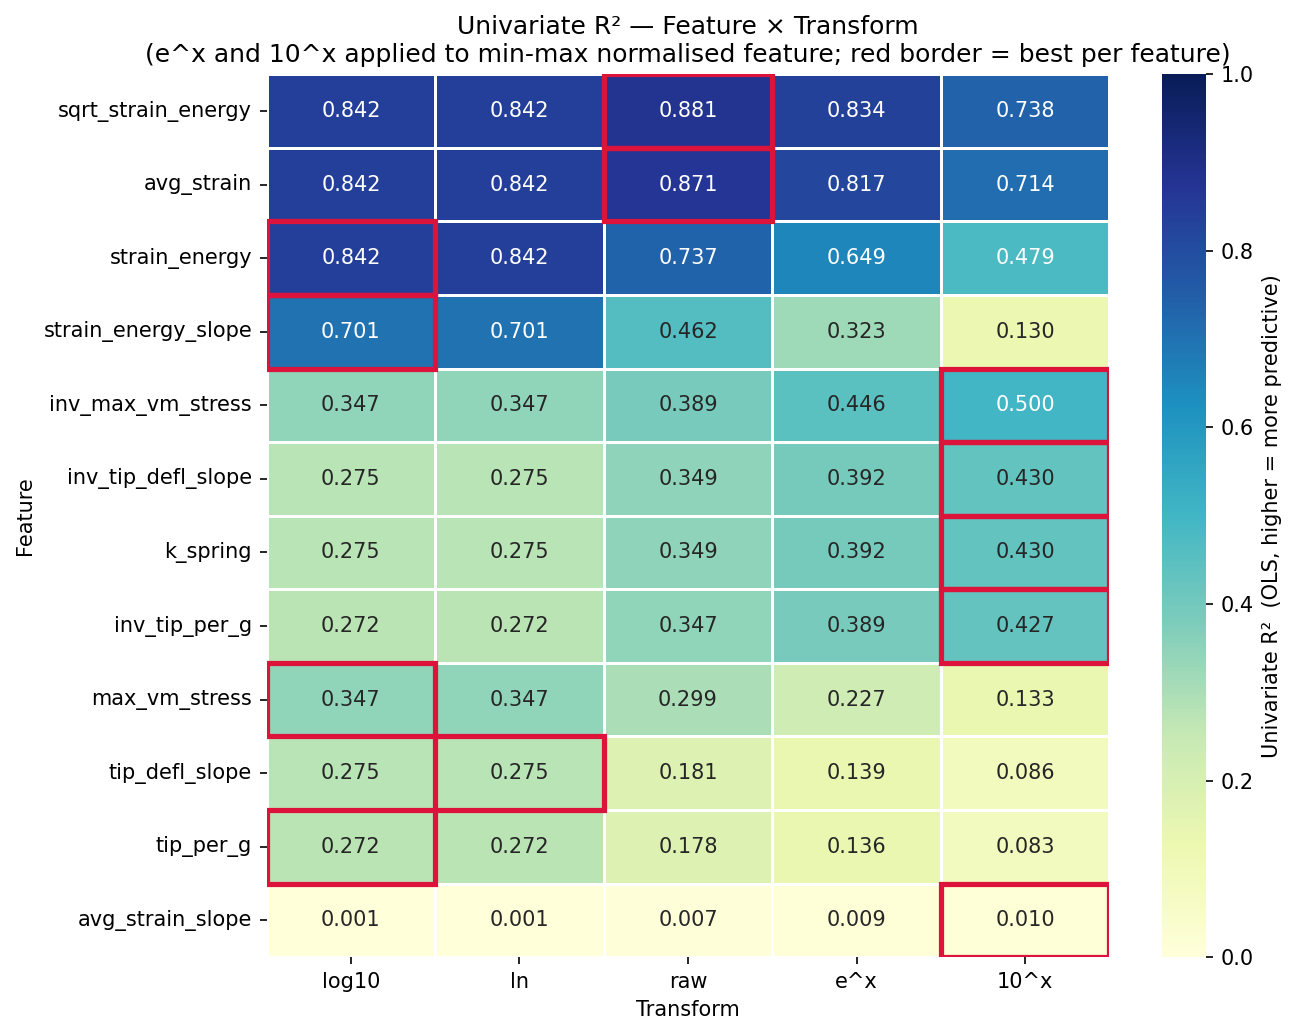
\includegraphics[width=\textwidth]{fig_07_transform_r2_heatmap.png}
  \caption{Heatmap of single-feature linear $\Rsq$ with $g$-limit across five transform
    types. Brighter cells indicate the best-performing transform per feature. Most features
    benefit from a log or Box-Cox compression; no single transform dominates across all
    features.}
  \label{fig:transform_heatmap}
\end{figure}

\begin{figure}[H]
  \centering
  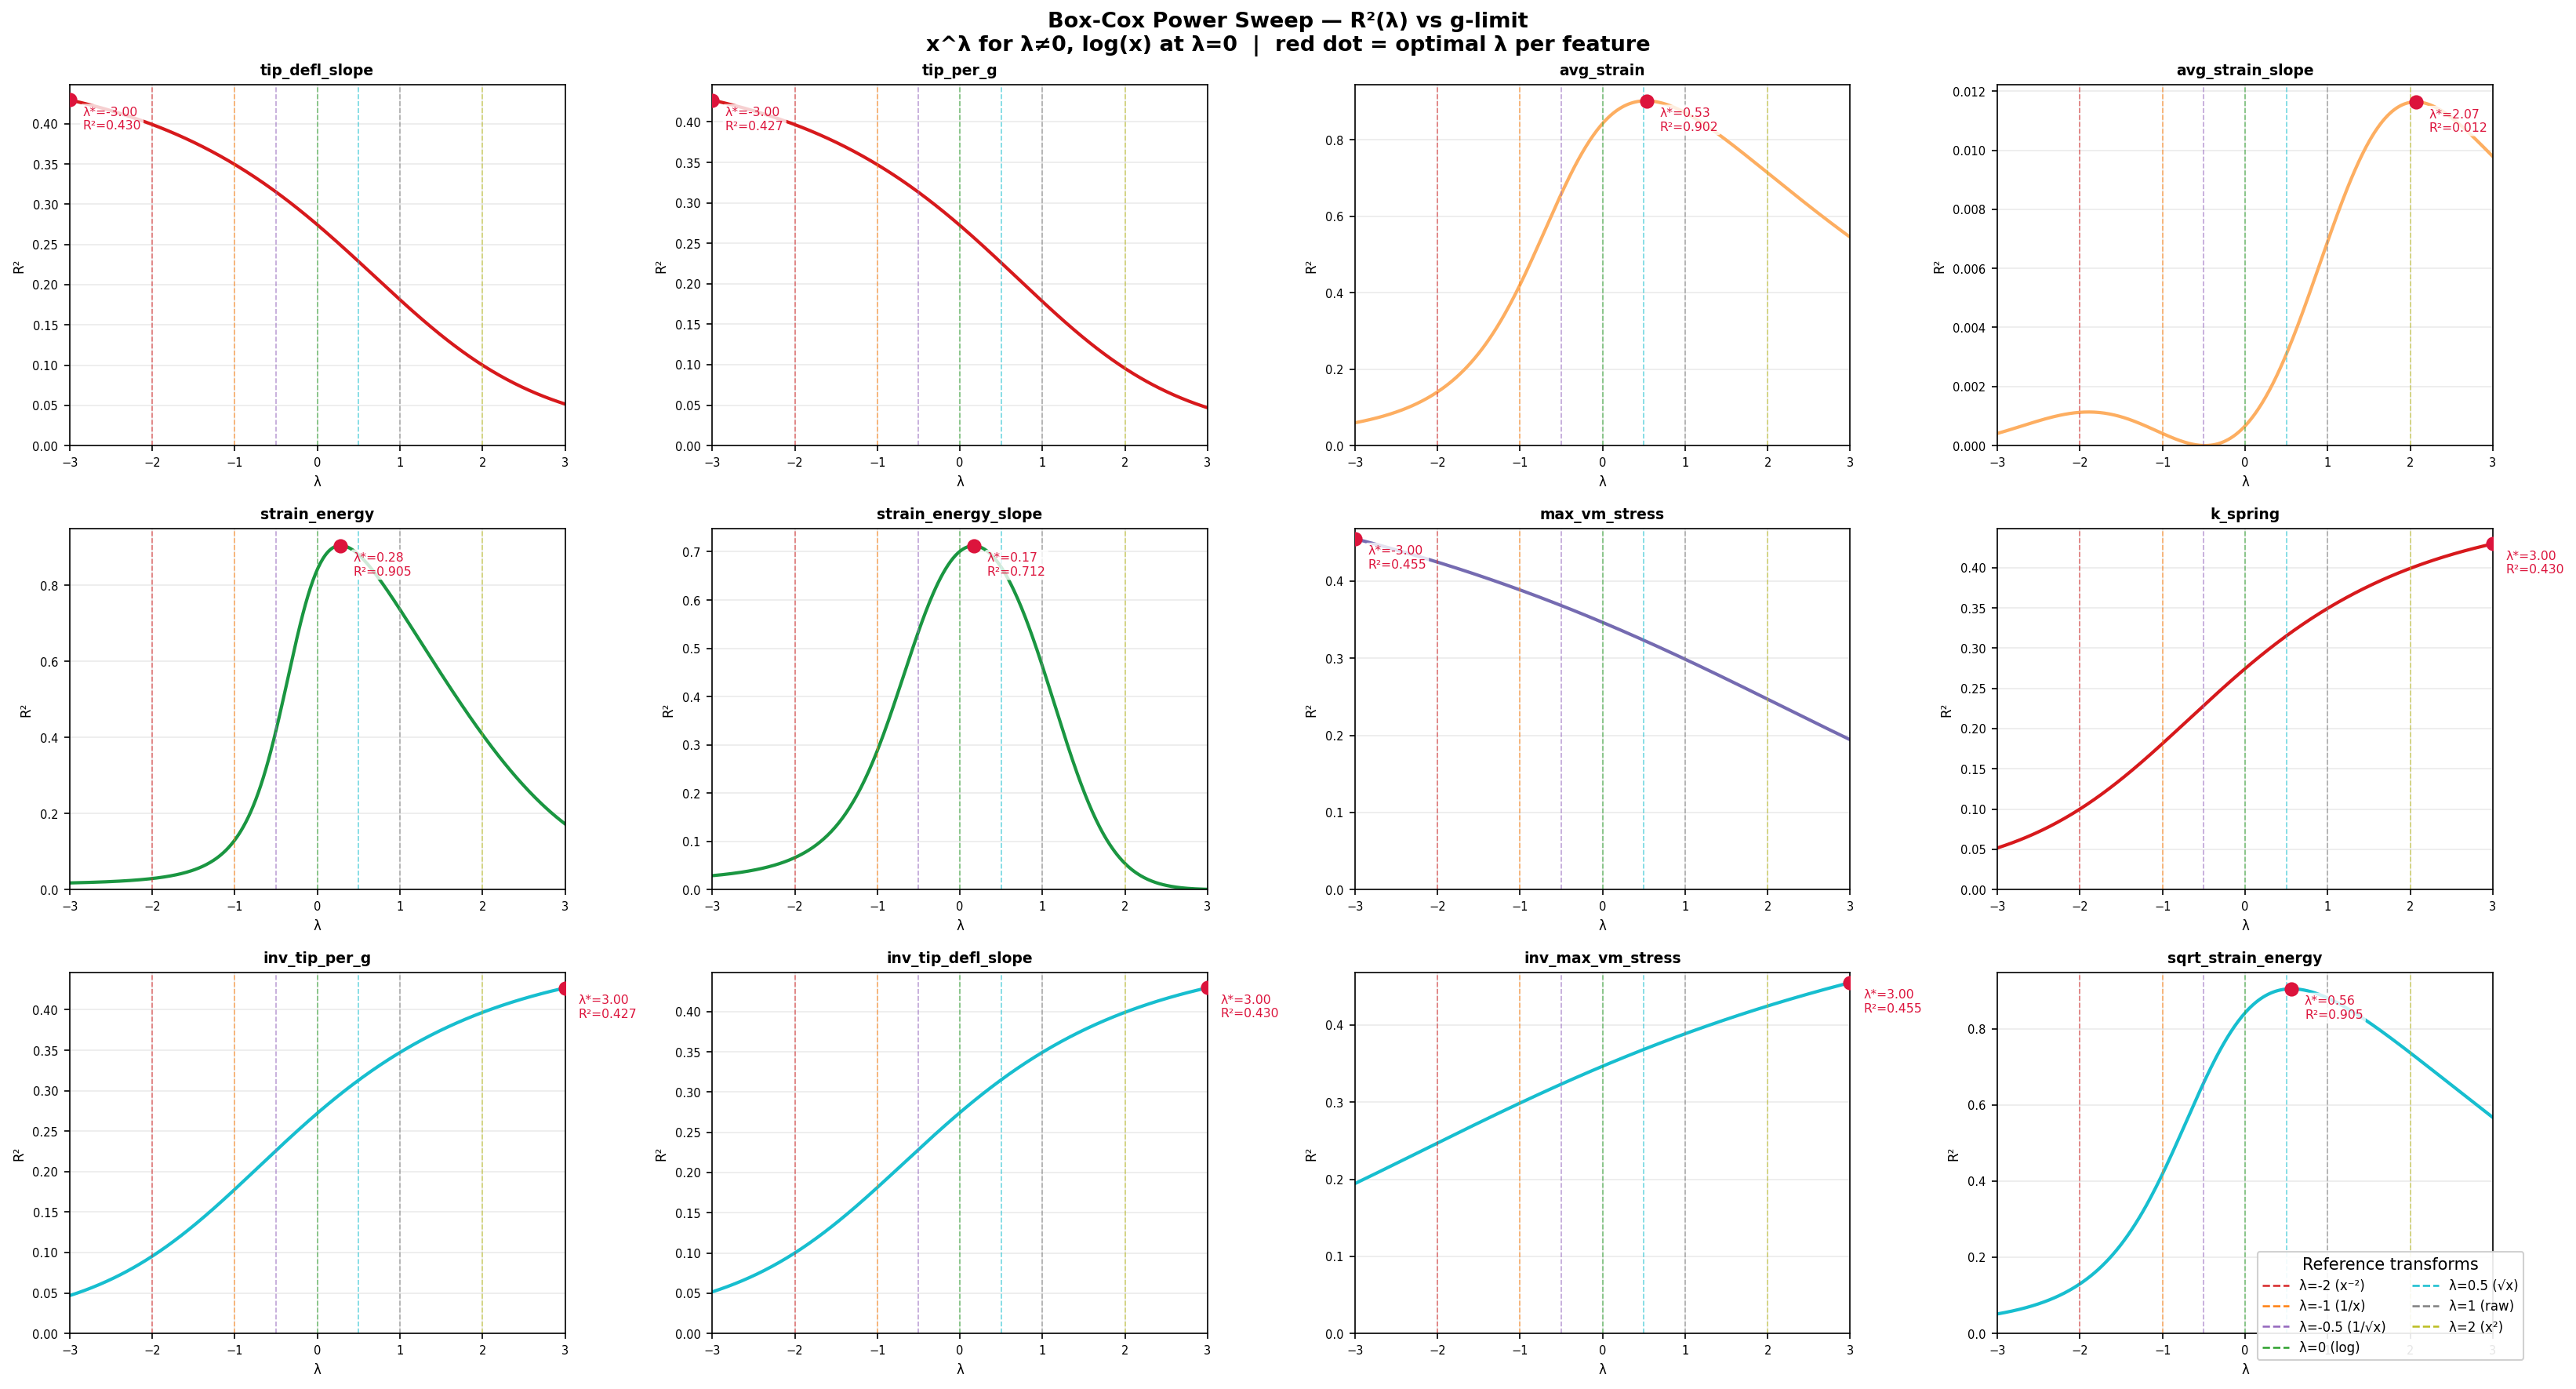
\includegraphics[width=\textwidth]{fig_08_boxcox_sweep.png}
  \caption{Box-Cox power $\lambda^*$ sweep for each engineered feature. Each curve shows how
    univariate $\Rsq$ changes as the exponent varies. The optimal $\lambda^*$ (marked) is used
    to construct the \texttt{boxcox\_*} feature columns.}
  \label{fig:boxcox_sweep}
\end{figure}

\subsubsection{Strain Gauge Rank Analysis}

Because the 24 strain gauge nodes have no fixed spatial correspondence across simulations
(each simulation has a different damage location and loading configuration), raw gauge
readings cannot be used as positionally-indexed features. To recover structure from this
unordered set, we sort each simulation's 24 at-failure strain values in ascending order,
assigning a within-simulation \textit{percentile rank} (rank~1 = lowest strain, rank~24 =
highest). This rank ordering is sufficient to produce a monotone, structured signal: the
rank-ordered median growth curve rises smoothly across all 468 simulations, and the per-rank
$\Rsq$ with $g$-limit is substantially higher than any unordered node-by-node $\Rsq$.

\textbf{Per-rank predictive power.} A single-feature linear regression on rank $k$ strain
achieves the $\Rsq$ values shown in Figure~\ref{fig:engineered_scatter}. The distribution is
bimodal: $\Rsq$ peaks near rank~4 ($\Rsq = 0.798$), drops through the middle ranks
($\Rsq \approx 0.70$ at ranks 8--10), then rises again to a global maximum at rank~23
($\Rsq = 0.885$). The rank-24 (highest strain) reading is slightly less predictive
($\Rsq = 0.861$), consistent with high variance from near-failure plasticity at the most
damaged locations. \textbf{No combination of spline-transformed features exceeds the rank-23
single-gauge predictor.}

\textbf{Continuous rank feature via spline inversion.} Rather than using the discrete
24-point strain values directly, we fitted parametric and interpolating curves to the median
rank-ordered growth profile and used each curve's inverse --- mapping each simulation's
actual strain to its implied rank position on the median curve --- as a continuous feature.
Eleven curve families were compared (logistic, cubic spline, PCHIP, Akima, least-squares
B-spline, Gompertz, Richards, Weibull CDF, power law, exponential, Hill). Among global
parametric forms, the \textbf{Gompertz curve} ($y = a\exp(-b\exp(-cx))$) best captures the
shape, achieving a median inverse-feature $\Rsq = 0.840$ vs.\ $0.798$ for the logistic. Its
asymmetric inflection (fixed at the lower third of the growth range by construction) matches
the observed accelerating-then-saturating strain profile better than the symmetric logistic.
Local interpolants (cubic spline, PCHIP, Akima) reach marginally higher peaks
($\Rsq \approx 0.880$) but offer no closed-form global description.

The spline-inversion approach does not outperform the best raw ranked gauge in peak $\Rsq$,
but it provides a more \textbf{uniform} predictor across all rank positions (median
$\Rsq \approx 0.808$ vs.\ a median of only $\approx 0.765$ across the 24 discrete ranks).
This is practically useful when the top-ranked gauge is noisy: the continuous inverse-spline
feature draws on information from the full rank profile rather than a single reading.

\begin{figure}[H]
  \centering
  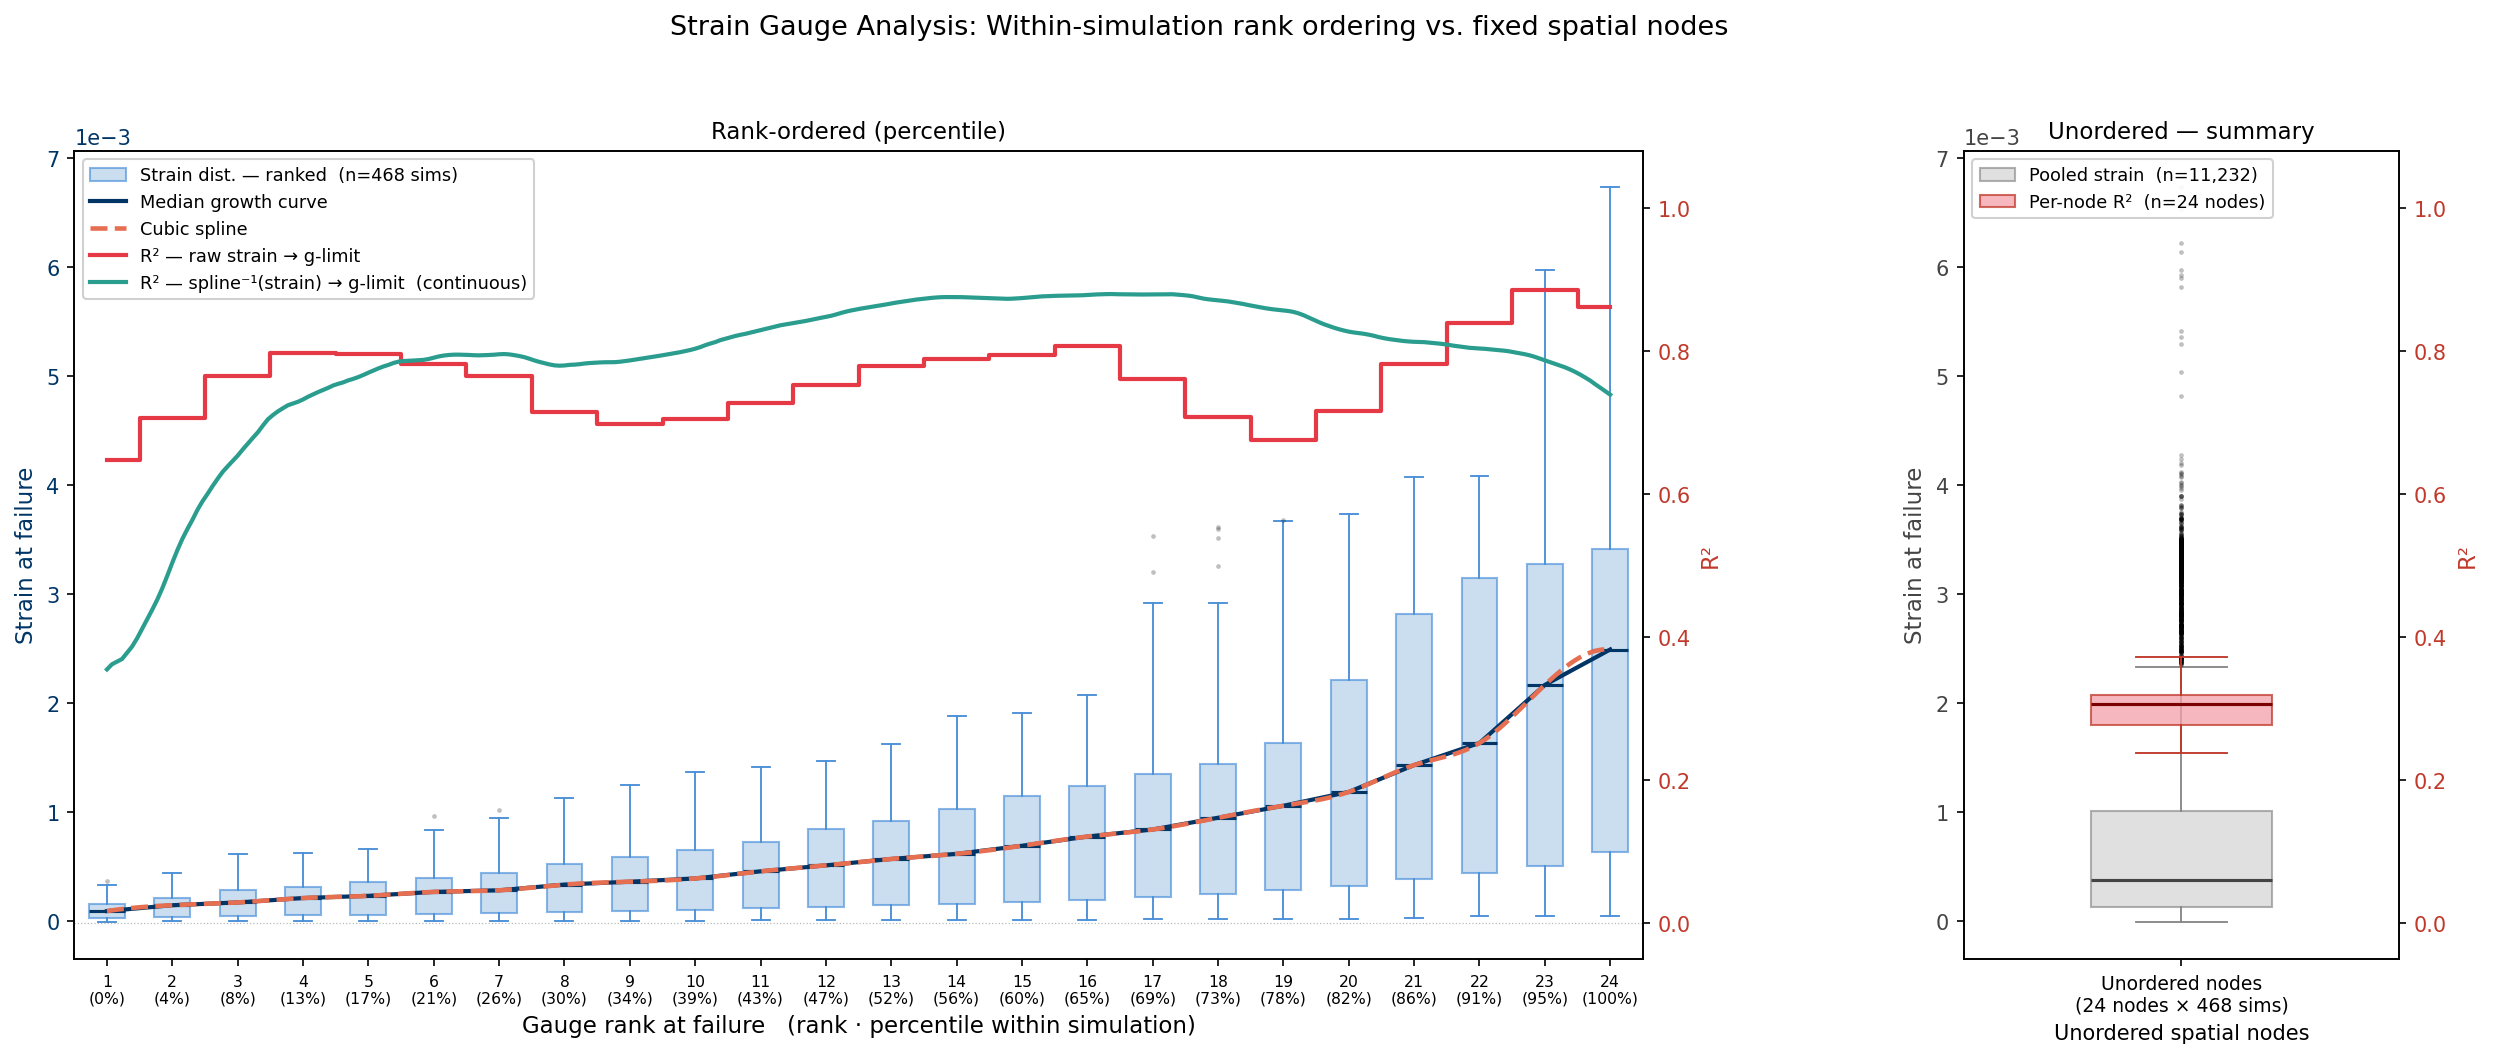
\includegraphics[width=\textwidth]{strain_gauge_rank_analysis.png}
  \caption{Left --- per-rank strain distributions (blue boxplots), median growth curve
    (navy), cubic spline overlay (orange dashed), and $\Rsq$ of raw rank-strain and
    spline-inverse feature vs.\ $g$-limit (right axis). Right --- pooled unordered-node
    strain distribution and per-node $\Rsq$ boxplot, demonstrating that rank ordering alone
    creates the structured monotone signal in the left panel.}
  \label{fig:rank_analysis}
\end{figure}

\subsection{Preprocessing}

\begin{enumerate}
  \item \textbf{Slope extraction:} Time-series load-ramp data were fit with a least-squares
    line to extract per-simulation slope features.
  \item \textbf{Strain energy:} Computed analytically from gauge readings, Young's modulus,
    and element volumes.
  \item \textbf{Normalization:} All features were standardized (zero mean, unit variance)
    using \texttt{sklearn.preprocessing.StandardScaler} fit on the training set only; the
    same scaler was applied to the test set.
  \item \textbf{LSTM padding:} Variable-length load ramps were zero-padded to the maximum
    sequence length (29 steps) and packed for efficient batch processing.
  \item \textbf{No data augmentation} was applied; the dataset represents a distinct ABAQUS
    simulation per sample.
\end{enumerate}

\subsection{Dataset Limitations}

\begin{itemize}
  \item Skin contribution to structural integrity is excluded; real $g$-limits will differ.
  \item Only static FEA; no dynamic loading or fatigue effects.
  \item Damage is modeled as clean cylindrical perforations; real ballistic damage includes
    petaling, cracking, and residual stress.
  \item No real flight data available for external validation.
\end{itemize}

% ============================================================
\section{Methods and System Implementation}
% ============================================================

Seven models were implemented in Python (scikit-learn + PyTorch) and evaluated on the same
dataset. All code is available in \texttt{models/} and \texttt{scripts/} in the project
repository.

\subsection{Classical Models}

\textbf{Model 1 --- Linear Regression} (\texttt{models/linear\_reg.py})
Standard ordinary least-squares regression on physics-engineered features with
\texttt{StandardScaler} normalization. Serves as the interpretable baseline.

\textit{Note on scaling requirement.} Box-Cox transforms span extreme numerical ranges
(e.g., \texttt{boxcox\_k\_spring} $\in [5\times10^{33},\, 10^{39}]$;
\texttt{boxcox\_max\_vm\_stress} $\in [10^{-107},\, 10^{-103}]$). Without
\texttt{StandardScaler}, sklearn's OLS solver sets the corresponding coefficients to zero and
silently discards those features. All results use \texttt{StandardScaler} fit on the training
set.

\textbf{Feature-set comparison (OLS $\Rsq$).}

\begin{table}[H]
  \caption{Linear Regression performance for key feature-set combinations. CV = 5-fold
    cross-validated $\Rsq$ on the training set.}
  \label{tab:lr_feats}
  \centering\small
  \begin{tabular}{@{}lccc@{}}
    \toprule
    \textbf{Feature Set} & \textbf{\# Features}
      & \textbf{In-sample $\Rsq$} & \textbf{5-fold CV $\Rsq$} \\
    \midrule
    \texttt{ranked\_strain\_p23} (best single feature) & 1  & 0.885 & 0.884 \\
    \texttt{RANKED\_STRAIN} (3 rank percentiles + Gompertz shape) & 5  & 0.906 & 0.900 \\
    \texttt{BOXCOX\_COLS\_LR} (6 non-collinear Box-Cox features)  & 6  & 0.966 & 0.964 \\
    Greedy-optimal (CV peak; see Figure~\ref{fig:pareto_features}) & 8  & 0.978 & \textbf{0.976} \\
    \texttt{BOXCOX\_COLS} (all 12 Box-Cox features)               & 12 & 0.976 & 0.972 \\
    \texttt{BOXCOX\_COLS + RANKED\_STRAIN} (full pool)            & 17 & 0.979 & 0.974 \\
    \bottomrule
  \end{tabular}
\end{table}

The CV $\Rsq$ peaks at $k=8$ under greedy forward selection
(Figure~\ref{fig:pareto_features}). Beyond that, additional features are collinear residuals:
in-sample $\Rsq$ increases by ${<}0.001$ while CV $\Rsq$ decreases slightly. The deployed
Linear Regression model uses \texttt{BOXCOX\_COLS\_LR} (6 features), selected before the
rank-ordered strain features were added; switching to the 8-feature greedy-optimal set would
improve CV $\Rsq$ from 0.964 to 0.976.

\textbf{Model 2 --- Polynomial Regression} (\texttt{models/poly\_reg.py})
Degree-2 polynomial expansion of the 7 engineered features (35 basis functions after
interaction terms), followed by ridge-regularized least-squares. Captures the nonlinear but
smooth $g$-limit--strain relationship.

\textbf{Model 3 --- Gaussian Process Regression} (\texttt{models/gpr.py})
GPR with a Mat\'{e}rn 5/2 kernel trained on the 12 Box-Cox optimal power-transformed
features. Provides a probabilistic prediction with calibrated uncertainty, naturally handling
the small dataset. The Box-Cox feature set pre-linearises the input space, which substantially
improves GP kernel fitting.

\textbf{Model 4 --- Random Forest} (\texttt{models/random\_forest.py})
Ensemble of 200 decision trees on all 31 features. Included as a non-parametric,
high-variance baseline to assess the value of ensemble methods on this dataset size.

\subsection{Modern Models}

\textbf{Model 5 --- Feedforward Neural Network (FFNN)}
(\texttt{models/feedforward\_nn.py})
Architecture: 31 inputs $\rightarrow$ [256, 128, 64] fully connected layers (ReLU,
dropout 0.2) $\rightarrow$ 1 output. Trained with Adam ($\text{lr}=10^{-3}$, weight
decay=$10^{-4}$), MSE loss, early stopping (patience=40 epochs). Best validation loss at
epoch 192.

\textbf{Model 6 --- Physics-Informed Neural Network (PINN)} (\texttt{models/pinn.py})
Same MLP architecture as the FFNN with an additional physics regularization term added to
the MSE loss:
\begin{equation}
  \mathcal{L} = \mathcal{L}_{\text{data}} + \lambda\,\mathcal{L}_{\text{physics}}
  \label{eq:pinn_loss}
\end{equation}

Three physics residuals were tested (ablation study in Section~\ref{sec:results}):
\begin{itemize}
  \item \textbf{Hooke strain:} $R_F = K_1 \times \varepsilon_{\text{avg}}$
    (linear elastic assumption)
  \item \textbf{Strain energy quadratic:} $R_F^2 = K_2 \times U$
    (elastic energy scales as $F^2$)
  \item \textbf{Energy rate (Castigliano):} $R_F = K_3 \times dU/dF$
    (Castigliano's theorem: tip deflection $\propto dU/dF \propto R_F/k$)
\end{itemize}

The best-performing variant was \textbf{energy\_rate} at $\lambda = 0.01$
($\adjRsq = 0.988$, RMSE$= 0.119$~g).

Each residual is normalized by the training-set standard deviation of the reference feature
so that $\lambda$ is dimensionless and comparable across physics models.

\textbf{Model 7 --- Deep Learning LSTM} (\texttt{models/deep\_learning.py})
Bidirectional LSTM (2 layers, hidden size 64) operating on raw time-series sensor data
(26 channels, $\leq$29 timesteps). Intended to exploit sequential load-ramp structure.
Trained with Adam, MSE loss, early stopping (patience=15 epochs). Stopped at epoch 31.

\subsection{End-to-End Pipeline}

\begin{figure}[H]
  \centering\small
  \texttt{ABAQUS simulation}
    \quad ($\downarrow$ Barrett Brown / Adam Zheng)\\[3pt]
  Raw \texttt{.csv} time-series (strain gauges, tip deflection, load)\\[3pt]
  $\downarrow$ \quad \texttt{data\_utils.py}\\[3pt]
  Feature engineering (7 scalars) + standardization\\[5pt]
  \begin{tabular}{@{}ccc@{}}
    \small$\swarrow$ & \hspace{2.5cm} & \small$\searrow$ \\[2pt]
    \texttt{train\_classical.py} & & \texttt{train\_modern.py} \\[2pt]
    \small$\searrow$ & \hspace{2.5cm} & \small$\swarrow$ \\
  \end{tabular}\\[3pt]
  \texttt{results/*.json}
    $\longleftarrow$ \texttt{evaluate.py} $\longrightarrow$ figures
  \caption{End-to-end data and training pipeline. All code is version-controlled in the
    project repository.}
  \label{fig:pipeline}
\end{figure}

\subsection{Software}

Python 3.12, NumPy, SciPy, scikit-learn 1.4, PyTorch 2.3; ABAQUS 2024 (FEA, Texas A\&M
HPRC FASTER cluster); Matplotlib 3.8 (figures).

% ============================================================
\section{Experimental Setup and Evaluation Metrics}
% ============================================================

\subsection{Evaluation Metrics}

Six metrics were computed for every model on the held-out test set:

\begin{table}[H]
  \caption{Evaluation metrics, symbols, and proposal thresholds.}
  \label{tab:metrics}
  \centering\small
  \begin{tabularx}{\textwidth}{@{}lllX@{}}
    \toprule
    \textbf{Metric} & \textbf{Symbol} & \textbf{Threshold} & \textbf{Description} \\
    \midrule
    Adjusted $\Rsq$       & $\adjRsq$  & $\geq 0.80$ &
      Fraction of variance explained, penalized for feature count \\
    Root Mean Square Error & RMSE      & $\leq 0.75$~g &
      RMS prediction error \\
    Mean Absolute Error    & MAE       & $\leq 0.50$~g &
      Average absolute prediction error \\
    Maximum overprediction & max-over  & ---           &
      Worst-case unsafe prediction \\
    Margin of Safety @ 1\%& MOS@1\%   & $\leq 0.25$~g &
      Safety buffer such that ${<}1\%$ of predictions exceed true $g$-limit \\
    Inference time         & $t_\text{infer}$ & ---   &
      Wall-clock time per prediction on laptop CPU (comparative only) \\
    \bottomrule
  \end{tabularx}
\end{table}

\textbf{MOS@1\%} is the primary safety metric: it is the smallest constant margin that,
when subtracted from all predictions, ensures fewer than 1\% of test cases would result in
an overprediction of the true $g$-limit. Smaller MOS means the model is both accurate and
well-calibrated from a safety standpoint.

\subsection{Baseline Strategy}

Linear Regression serves as the primary interpretable baseline. All other models are compared
against it and against the proposal success thresholds. The LSTM additionally serves as an
upper bound on what raw time-series data can contribute.

\subsection{PINN Ablation}

A full grid search over 3 physics models $\times$ 10 $\lambda$ values (0.001 to 30) was
conducted to determine the optimal physics-loss weighting. Each configuration was trained
with the same early stopping and architecture.

\subsection{Cross-Validation}

Classical models were evaluated with 5-fold cross-validated $\Rsq$ on the training set in
addition to the test-set metrics, to detect overfitting.

% ============================================================
\section{Results}
\label{sec:results}
% ============================================================

\subsection{Model Comparison Summary}

\begin{table}[H]
  \caption{Test-set performance across all seven models. Best value in each column is bold.}
  \label{tab:comparison}
  \centering\small
  \resizebox{\textwidth}{!}{%
  \begin{tabular}{@{}lcccccc@{}}
    \toprule
    \textbf{Model}
      & $\adjRsq$
      & \textbf{RMSE (g)}
      & \textbf{MAE (g)}
      & \textbf{Max Overpred.\ (g)}
      & \textbf{MOS@1\% (g)}
      & \textbf{Infer.\ (ms)} \\
    \midrule
    \textbf{GPR}
      & \textbf{0.9997} & \textbf{0.021} & \textbf{0.007}
      & \textbf{0.181} & \textbf{0.078} & 1.2 \\
    Poly Reg.
      & 0.994 & 0.100 & 0.070 & 0.211 & 0.156 & \textbf{0.24} \\
    Feedforward NN
      & 0.988 & 0.121 & 0.094 & 0.356 & 0.329 & 3.7 \\
    PINN (energy-rate, $\lambda\!=\!0.01$)
      & 0.988 & 0.122 & 0.095 & 0.346 & 0.330 & 2.6 \\
    Linear Reg.
      & 0.970 & 0.226 & 0.181 & 0.650 & 0.644 & 0.09 \\
    Random Forest
      & 0.956 & 0.229 & 0.137 & 0.885 & 0.729 & 57.9 \\
    LSTM
      & 0.862 & 0.413 & 0.232 & 2.327 & 0.826 & 152.2 \\
    \bottomrule
  \end{tabular}}
\end{table}

\begin{table}[H]
  \caption{Proposal success-criteria satisfaction (\cmark{} = meets threshold,
    \xmark{} = does not meet).}
  \label{tab:criteria}
  \centering\small
  \begin{tabular}{@{}lcccc@{}}
    \toprule
    \textbf{Model}
      & $\adjRsq \geq 0.80$
      & RMSE $\leq 0.75$~g
      & MAE $\leq 0.50$~g
      & MOS@1\% $\leq 0.25$~g \\
    \midrule
    GPR          & \cmark & \cmark & \cmark & \cmark~(0.078) \\
    Poly Reg.    & \cmark & \cmark & \cmark & \cmark~(0.156) \\
    FFNN         & \cmark & \cmark & \cmark & \xmark~(0.329) \\
    PINN         & \cmark & \cmark & \cmark & \xmark~(0.330) \\
    Lin.\ Reg.   & \cmark & \cmark & \cmark & \xmark~(0.644) \\
    Rand.\ Forest& \cmark & \cmark & \cmark & \xmark~(0.729) \\
    LSTM         & \cmark & \cmark & \cmark & \xmark~(0.826) \\
    \bottomrule
  \end{tabular}
\end{table}

\textbf{GPR and Polynomial Regression are the only models meeting all four success criteria.
GPR leads on every metric; Polynomial Regression is the best non-probabilistic model.}

\begin{figure}[H]
  \centering
  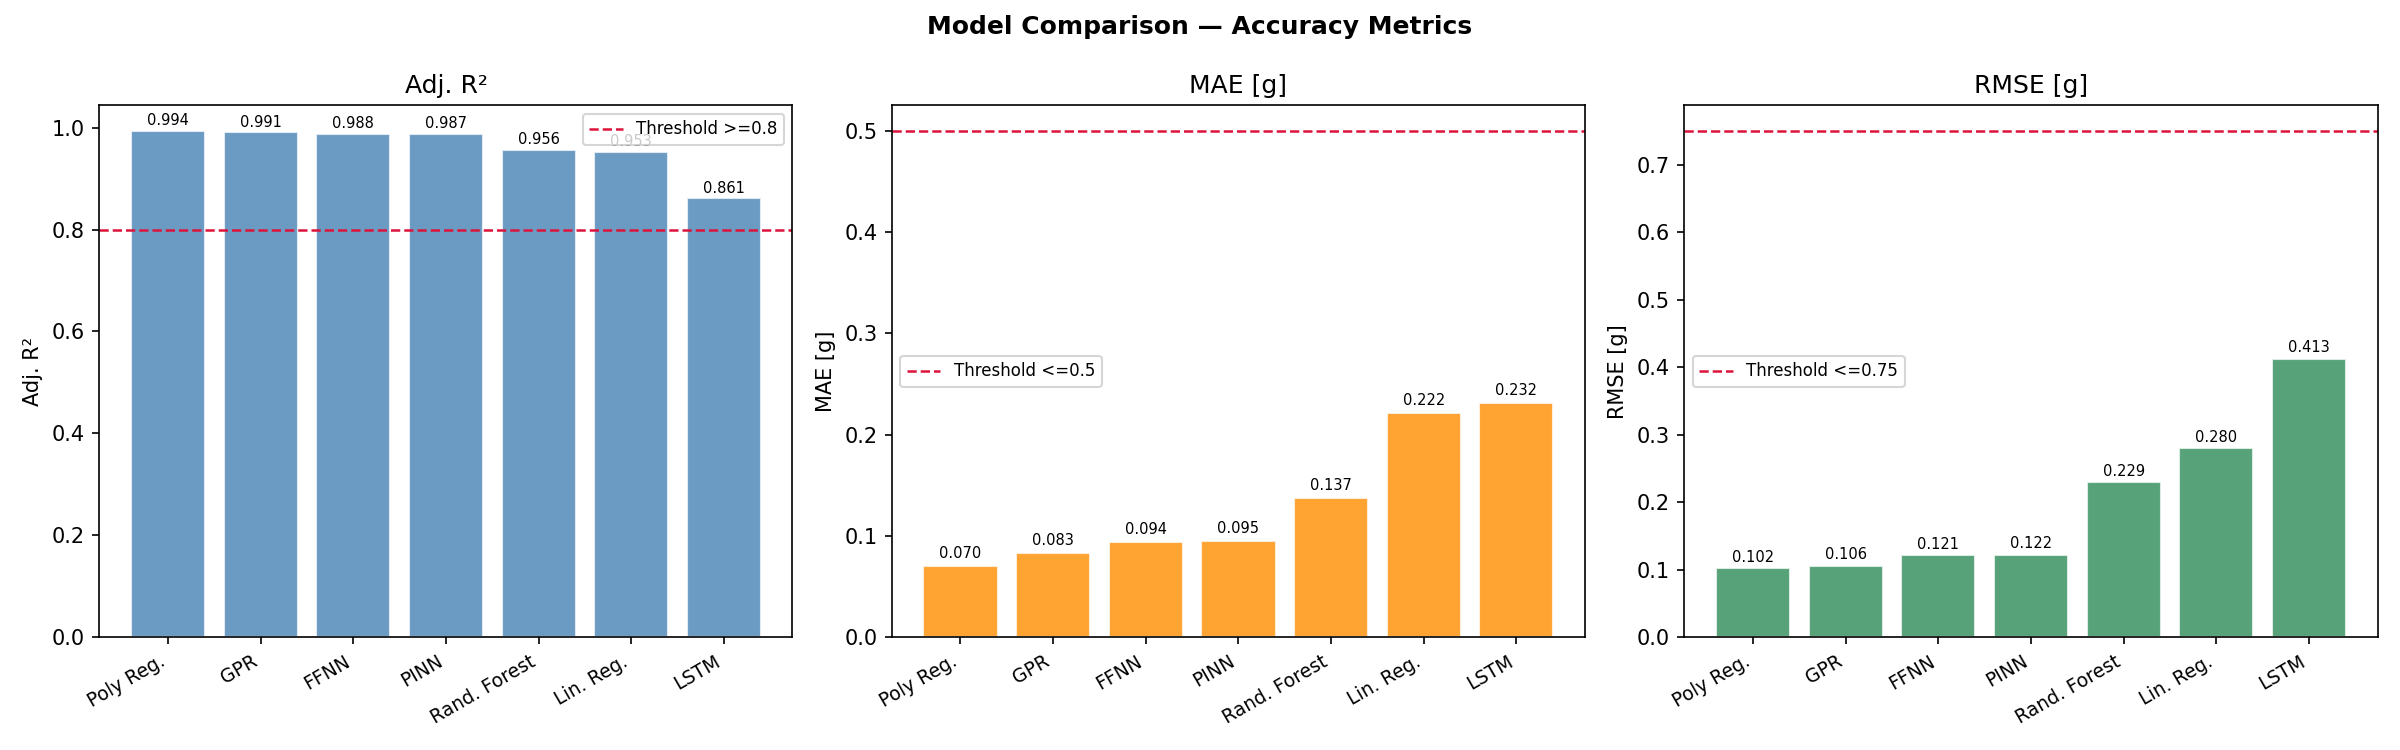
\includegraphics[width=\textwidth]{comparison_bar.png}
  \caption{Model performance comparison. GPR leads on all accuracy metrics; Polynomial
    Regression is the best interpretable non-probabilistic model.}
  \label{fig:comparison_bar}
\end{figure}

\begin{figure}[H]
  \centering
  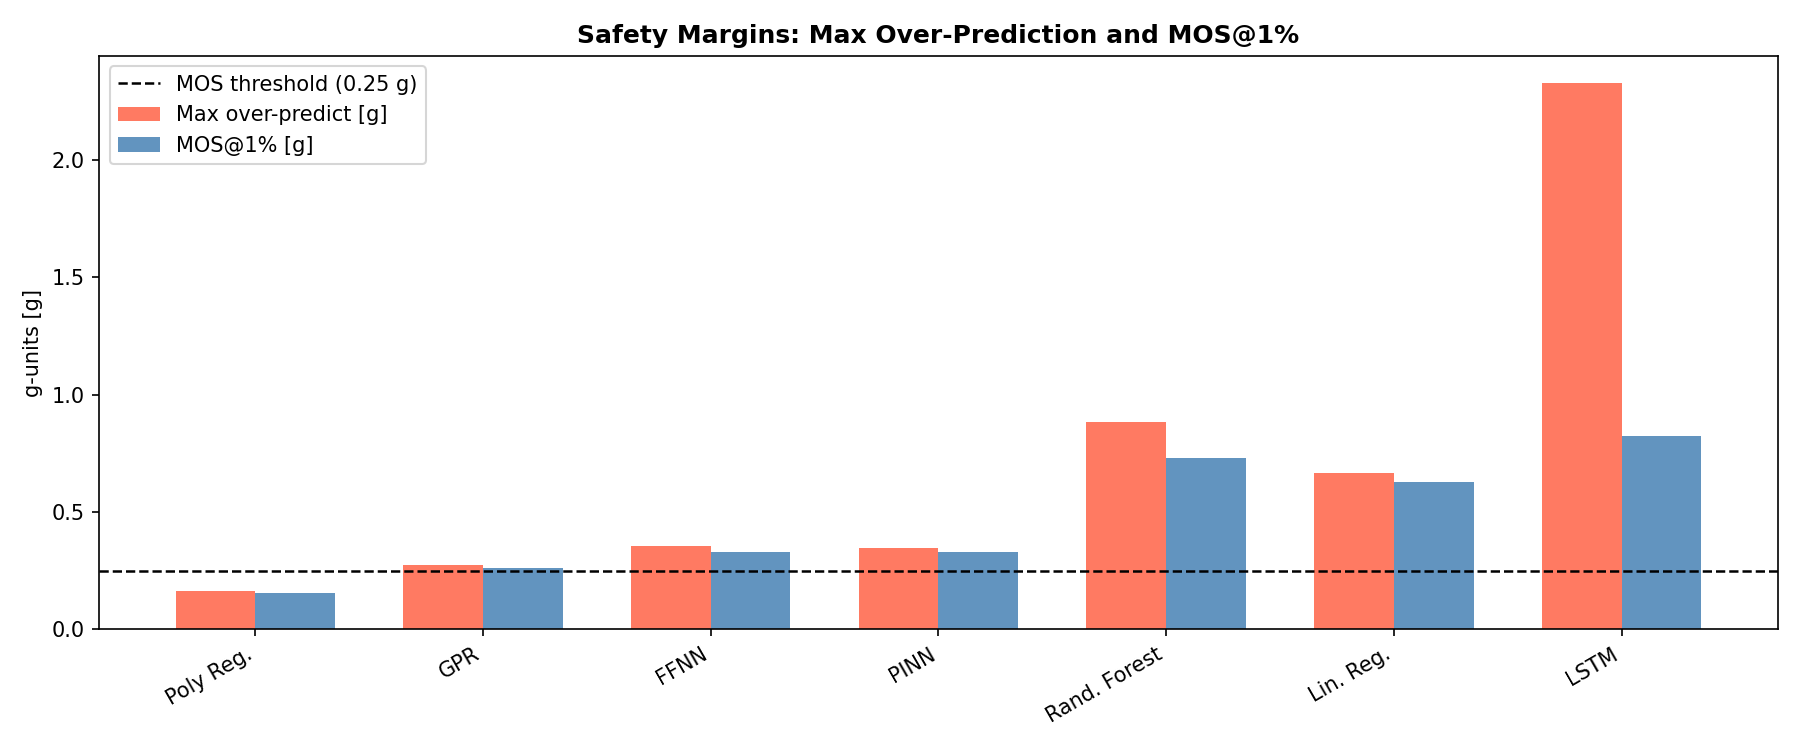
\includegraphics[width=0.85\textwidth]{comparison_mos.png}
  \caption{Safety metric comparison. The dashed line marks the MOS@1\% $= 0.25$~g
    threshold from the proposal. GPR and Polynomial Regression both fall below it.}
  \label{fig:comparison_mos}
\end{figure}

\subsection{Predicted vs.\ True and Residual Analysis}

\begin{figure}[H]
  \centering
  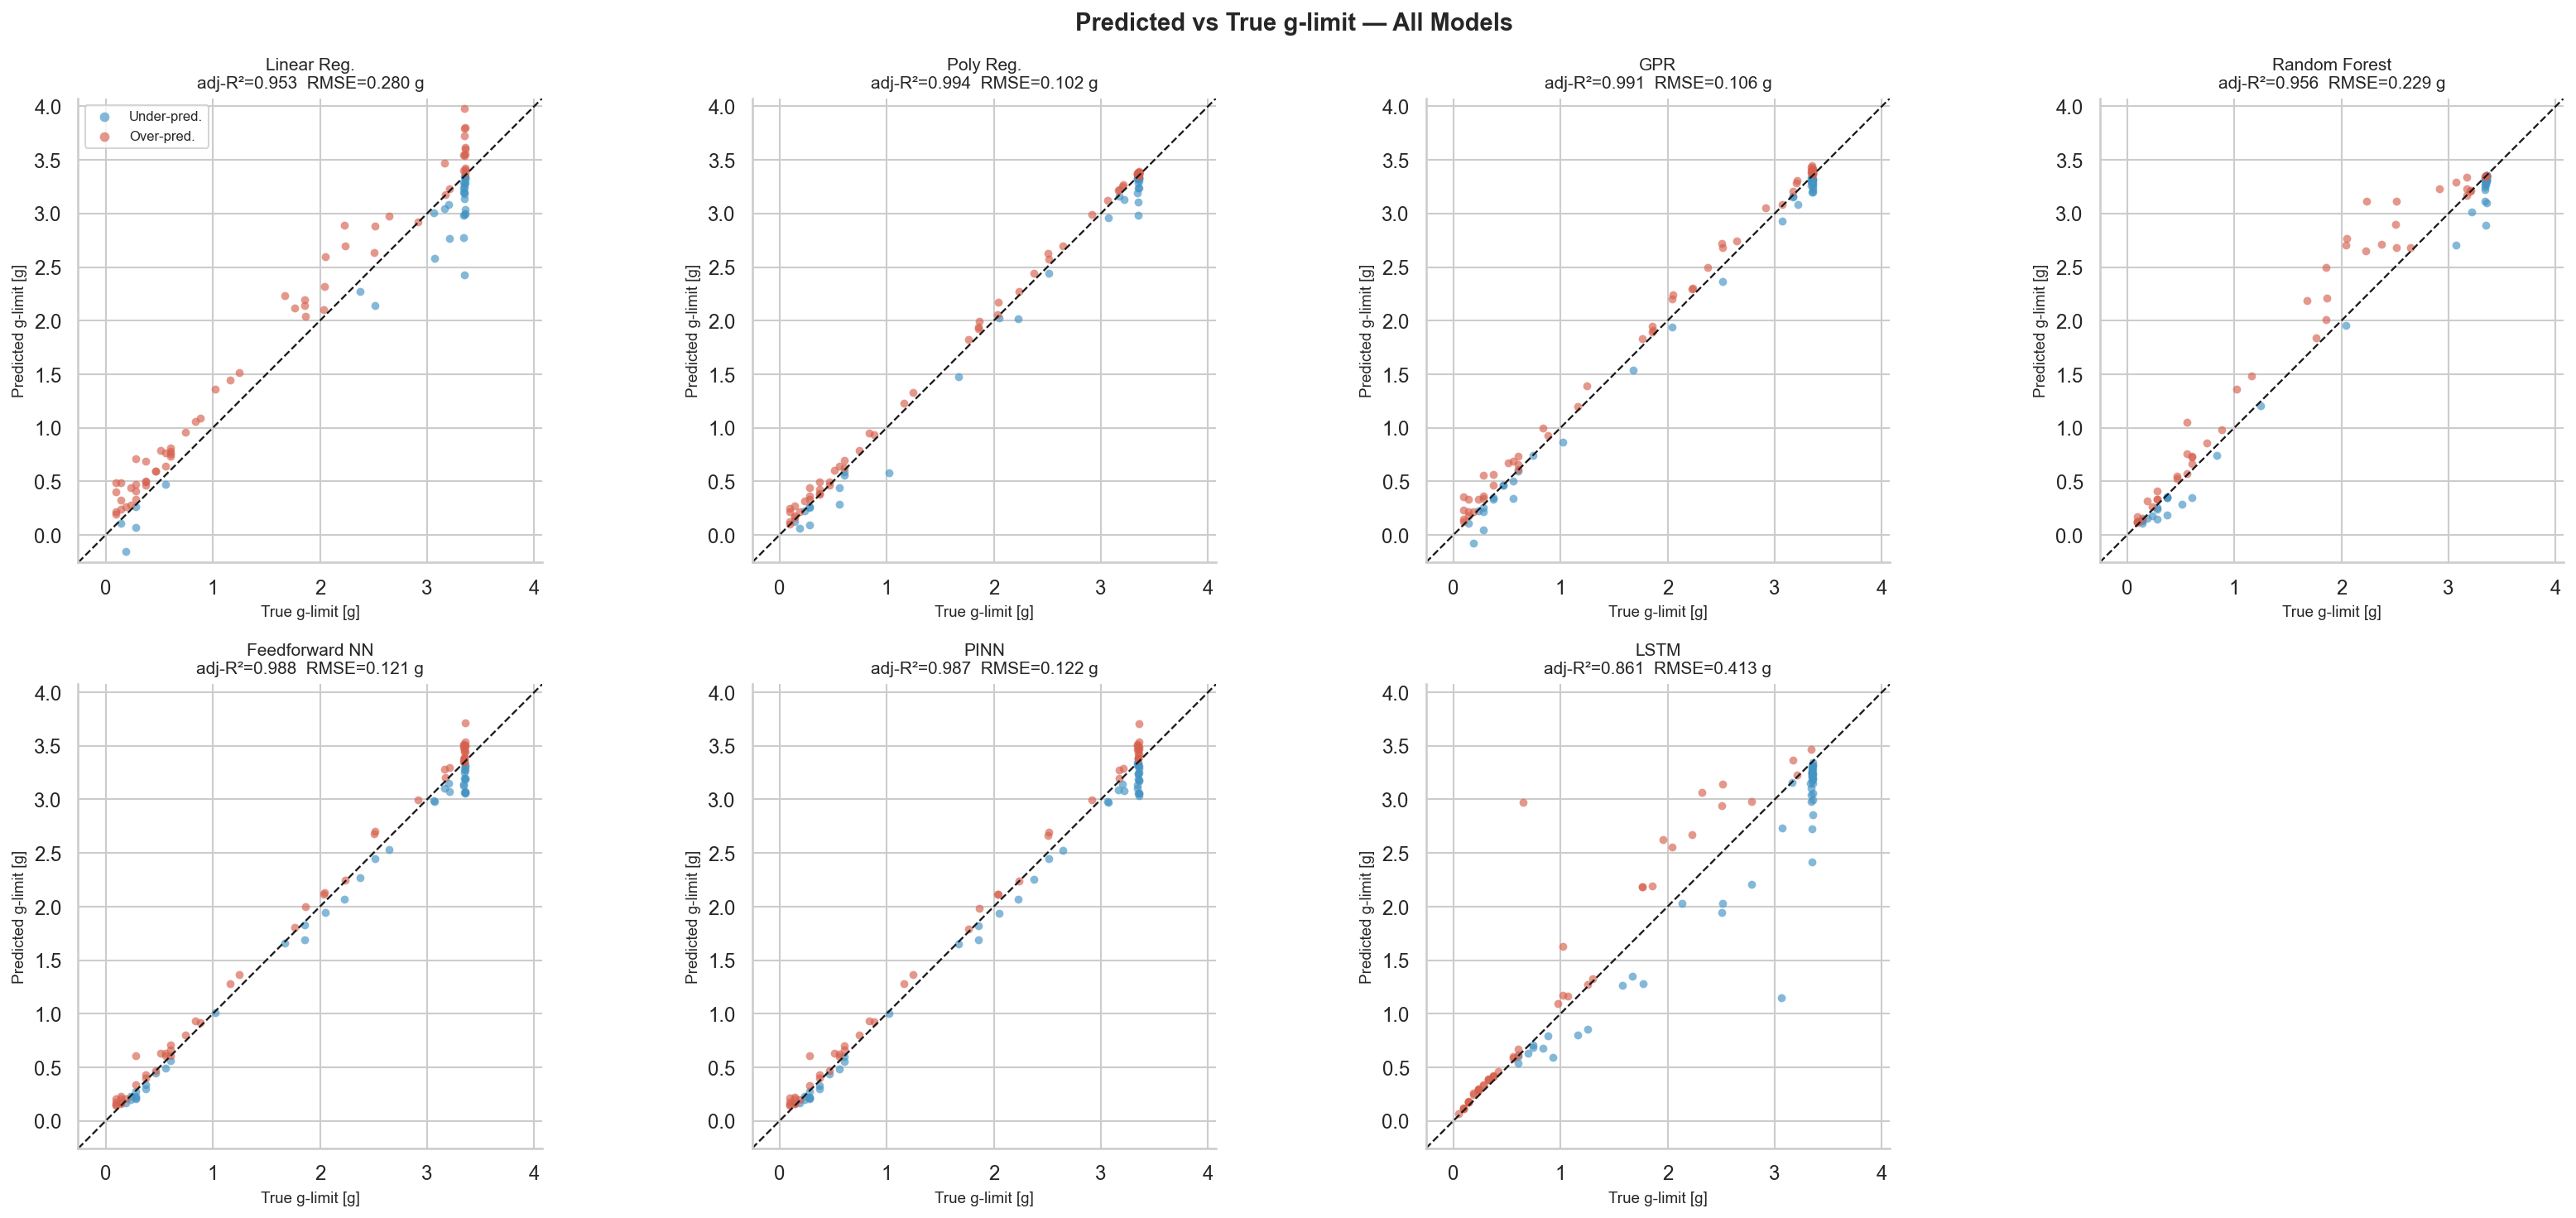
\includegraphics[width=\textwidth]{pred_vs_true.png}
  \caption{Predicted vs.\ true $g$-limit plots for each model. GPR and Polynomial Regression
    show tight clustering along the diagonal. LSTM shows systematic bias at extreme
    $g$-limits.}
  \label{fig:pred_vs_true}
\end{figure}

\begin{figure}[H]
  \centering
  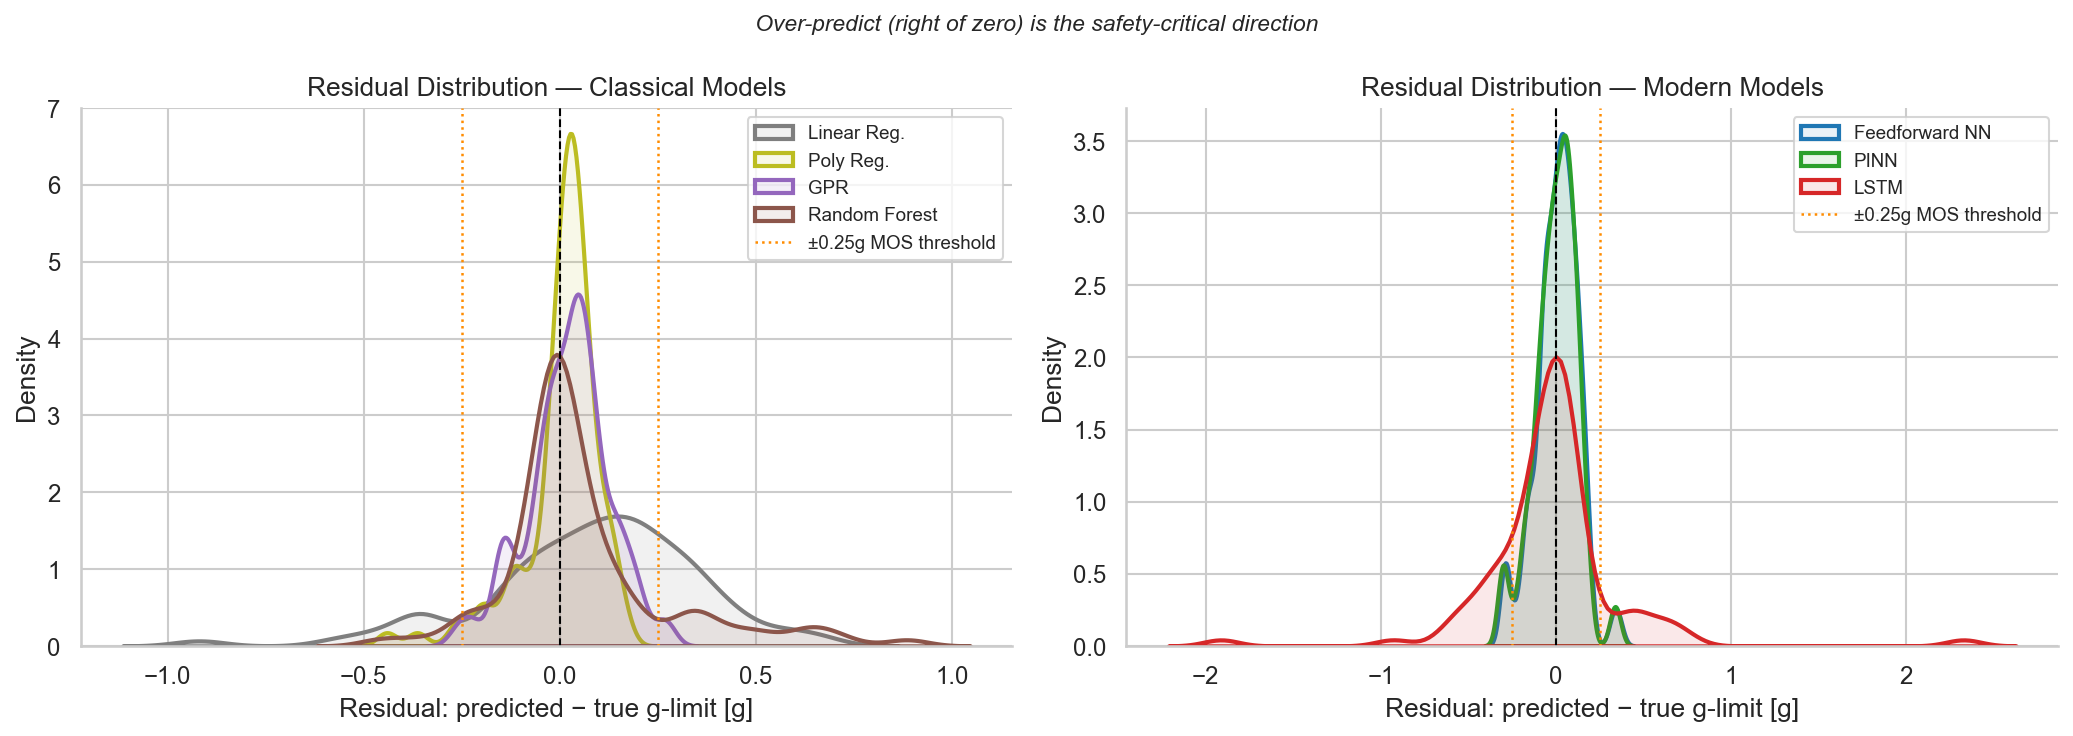
\includegraphics[width=\textwidth]{residual_dist.png}
  \caption{Residual (predicted $-$ true) distributions. GPR and Polynomial Regression are
    centered near zero with narrow spread. Random Forest shows a right tail indicating
    occasional large overpredictions.}
  \label{fig:residual_dist}
\end{figure}

\begin{figure}[H]
  \centering
  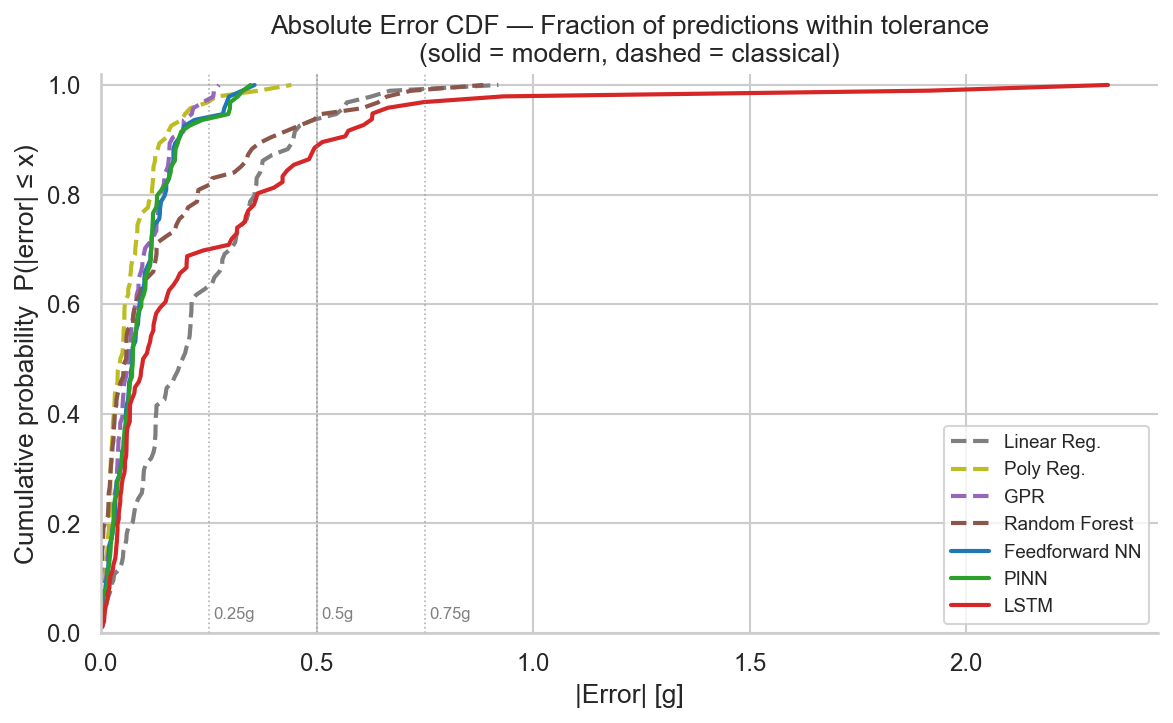
\includegraphics[width=0.85\textwidth]{abs_error_cdf.png}
  \caption{CDF of absolute test errors. GPR achieves the smallest errors across the full
    distribution; Polynomial Regression is the second best.}
  \label{fig:abs_error_cdf}
\end{figure}

\begin{figure}[H]
  \centering
  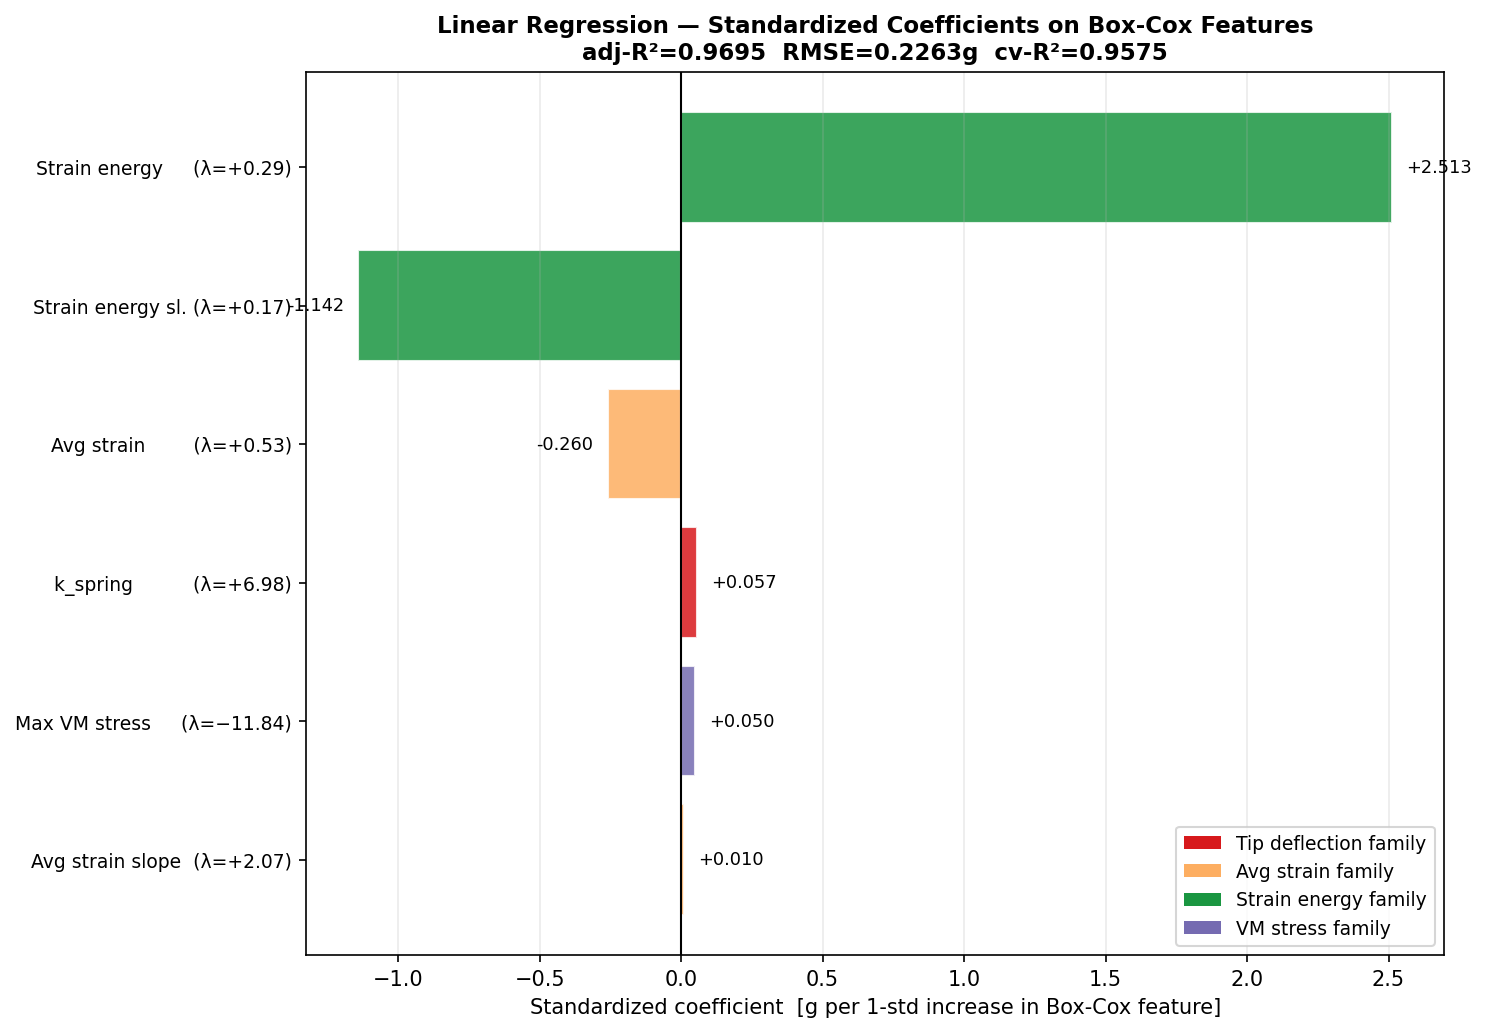
\includegraphics[width=0.85\textwidth]{lr_coefficients.png}
  \caption{Standardized coefficients for Linear Regression on the 6-feature Box-Cox set.
    Each bar shows the change in predicted $g$-limit per one-standard-deviation increase in
    the corresponding Box-Cox-transformed feature. Avg strain slope and max VM stress
    dominate; \texttt{k\_spring} provides a distinct structural-stiffness contribution.
    Features that grow as damage increases carry negative coefficients (reduced $g$-limit),
    consistent with physical expectation.}
  \label{fig:lr_coefficients}
\end{figure}

\begin{figure}[H]
  \centering
  
\includegraphics[width=0.85\textwidth]{poly_coefficients.png}
  \caption{Standardized coefficients for Polynomial Regression (degree-2 Ridge) on the 12
    Box-Cox features, sorted by absolute magnitude. Blue = linear terms, red = pure
    quadratic terms (e.g.\ avg\_strain$^2$), teal = cross-product interaction terms. The
    dominant linear terms (avg strain slope, max VM stress) mirror the Linear Regression
    hierarchy; quadratic and interaction terms with avg strain provide the nonlinear
    correction that closes the accuracy gap from $\adjRsq = 0.970$ to $0.994$.}
  \label{fig:poly_coefficients}
\end{figure}

\subsection{Safety Analysis}

\begin{figure}[H]
  \centering
  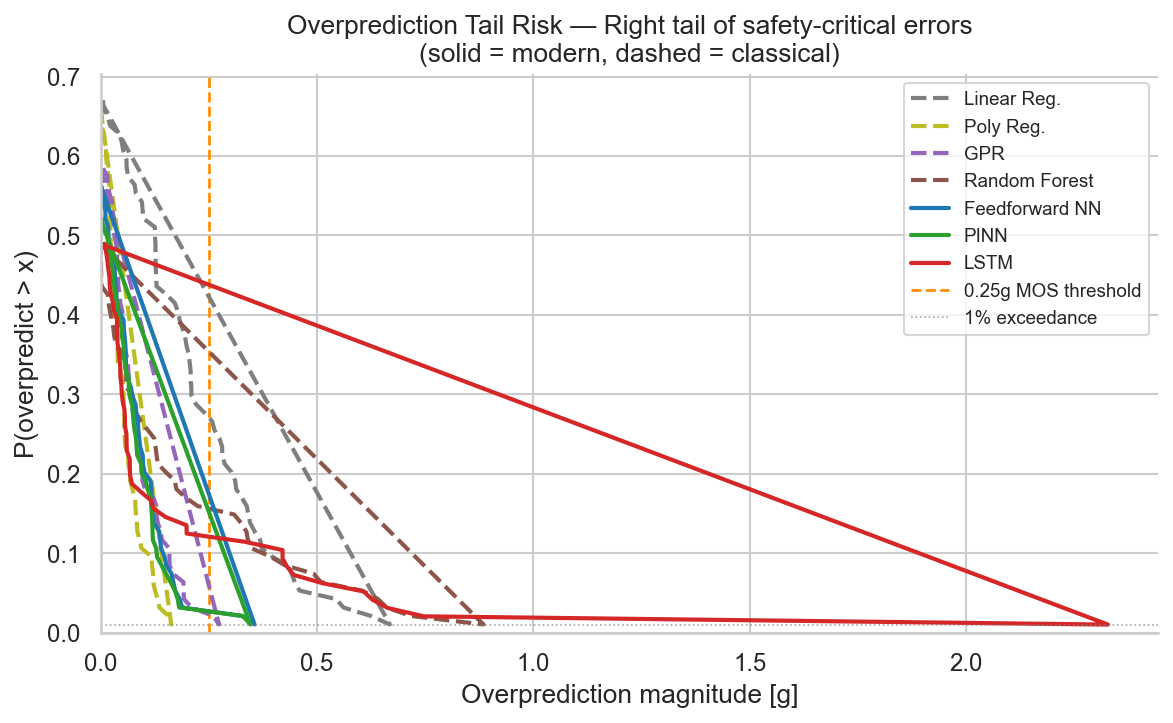
\includegraphics[width=0.85\textwidth]{overpredict_cdf.png}
  \caption{Overprediction CDF. At the MOS@1\% threshold (vertical marker), GPR
    (MOS $= 0.078$~g) and Polynomial Regression (MOS $= 0.156$~g) both satisfy the
    ${<}1\%$ overprediction requirement with a margin below 0.25~g.}
  \label{fig:overpredict_cdf}
\end{figure}

\begin{figure}[H]
  \centering
  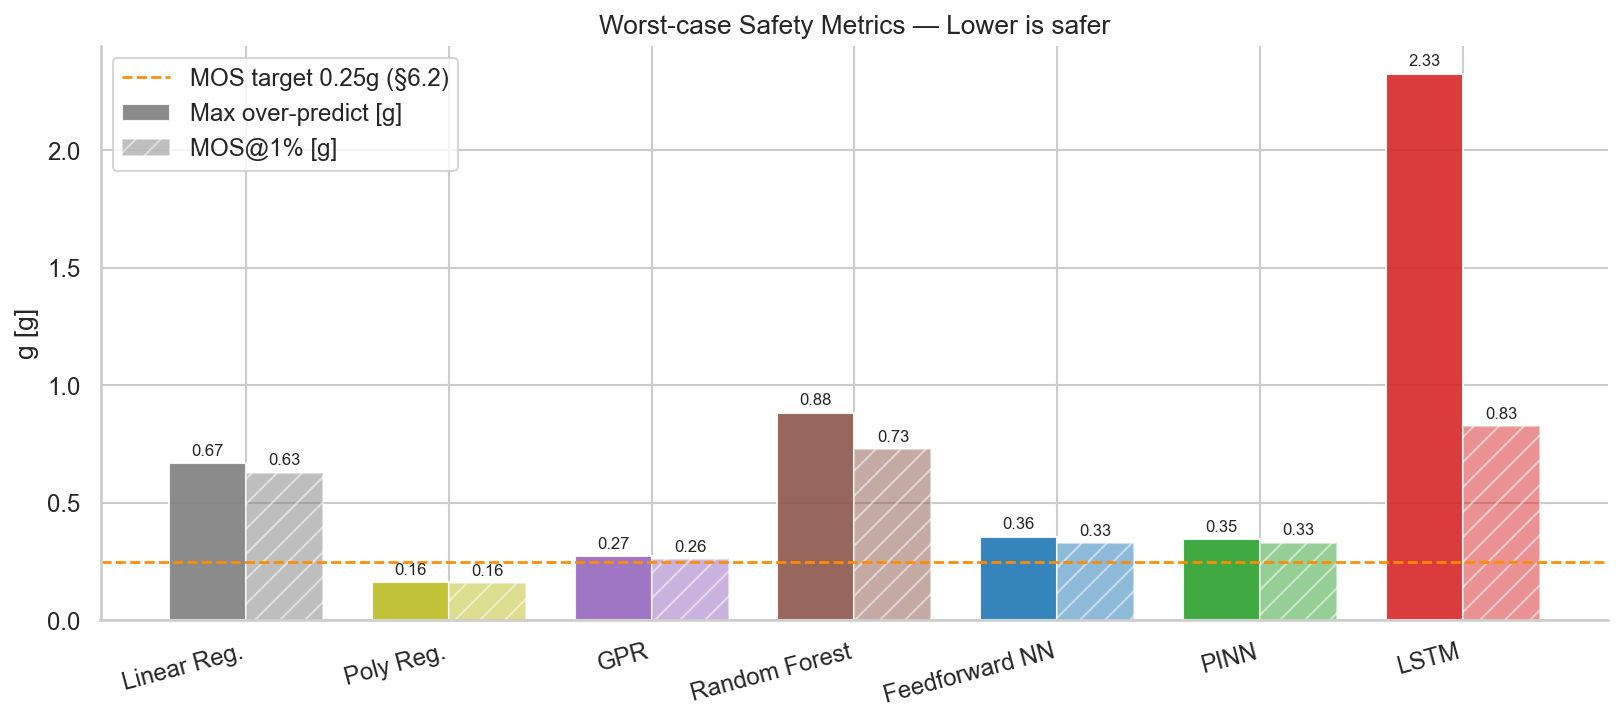
\includegraphics[width=0.85\textwidth]{safety_bars.png}
  \caption{Safety bar summary. GPR and Polynomial Regression (leftmost bars) are the only
    models below the 0.25~g MOS threshold.}
  \label{fig:safety_bars}
\end{figure}

\begin{figure}[H]
  \centering
  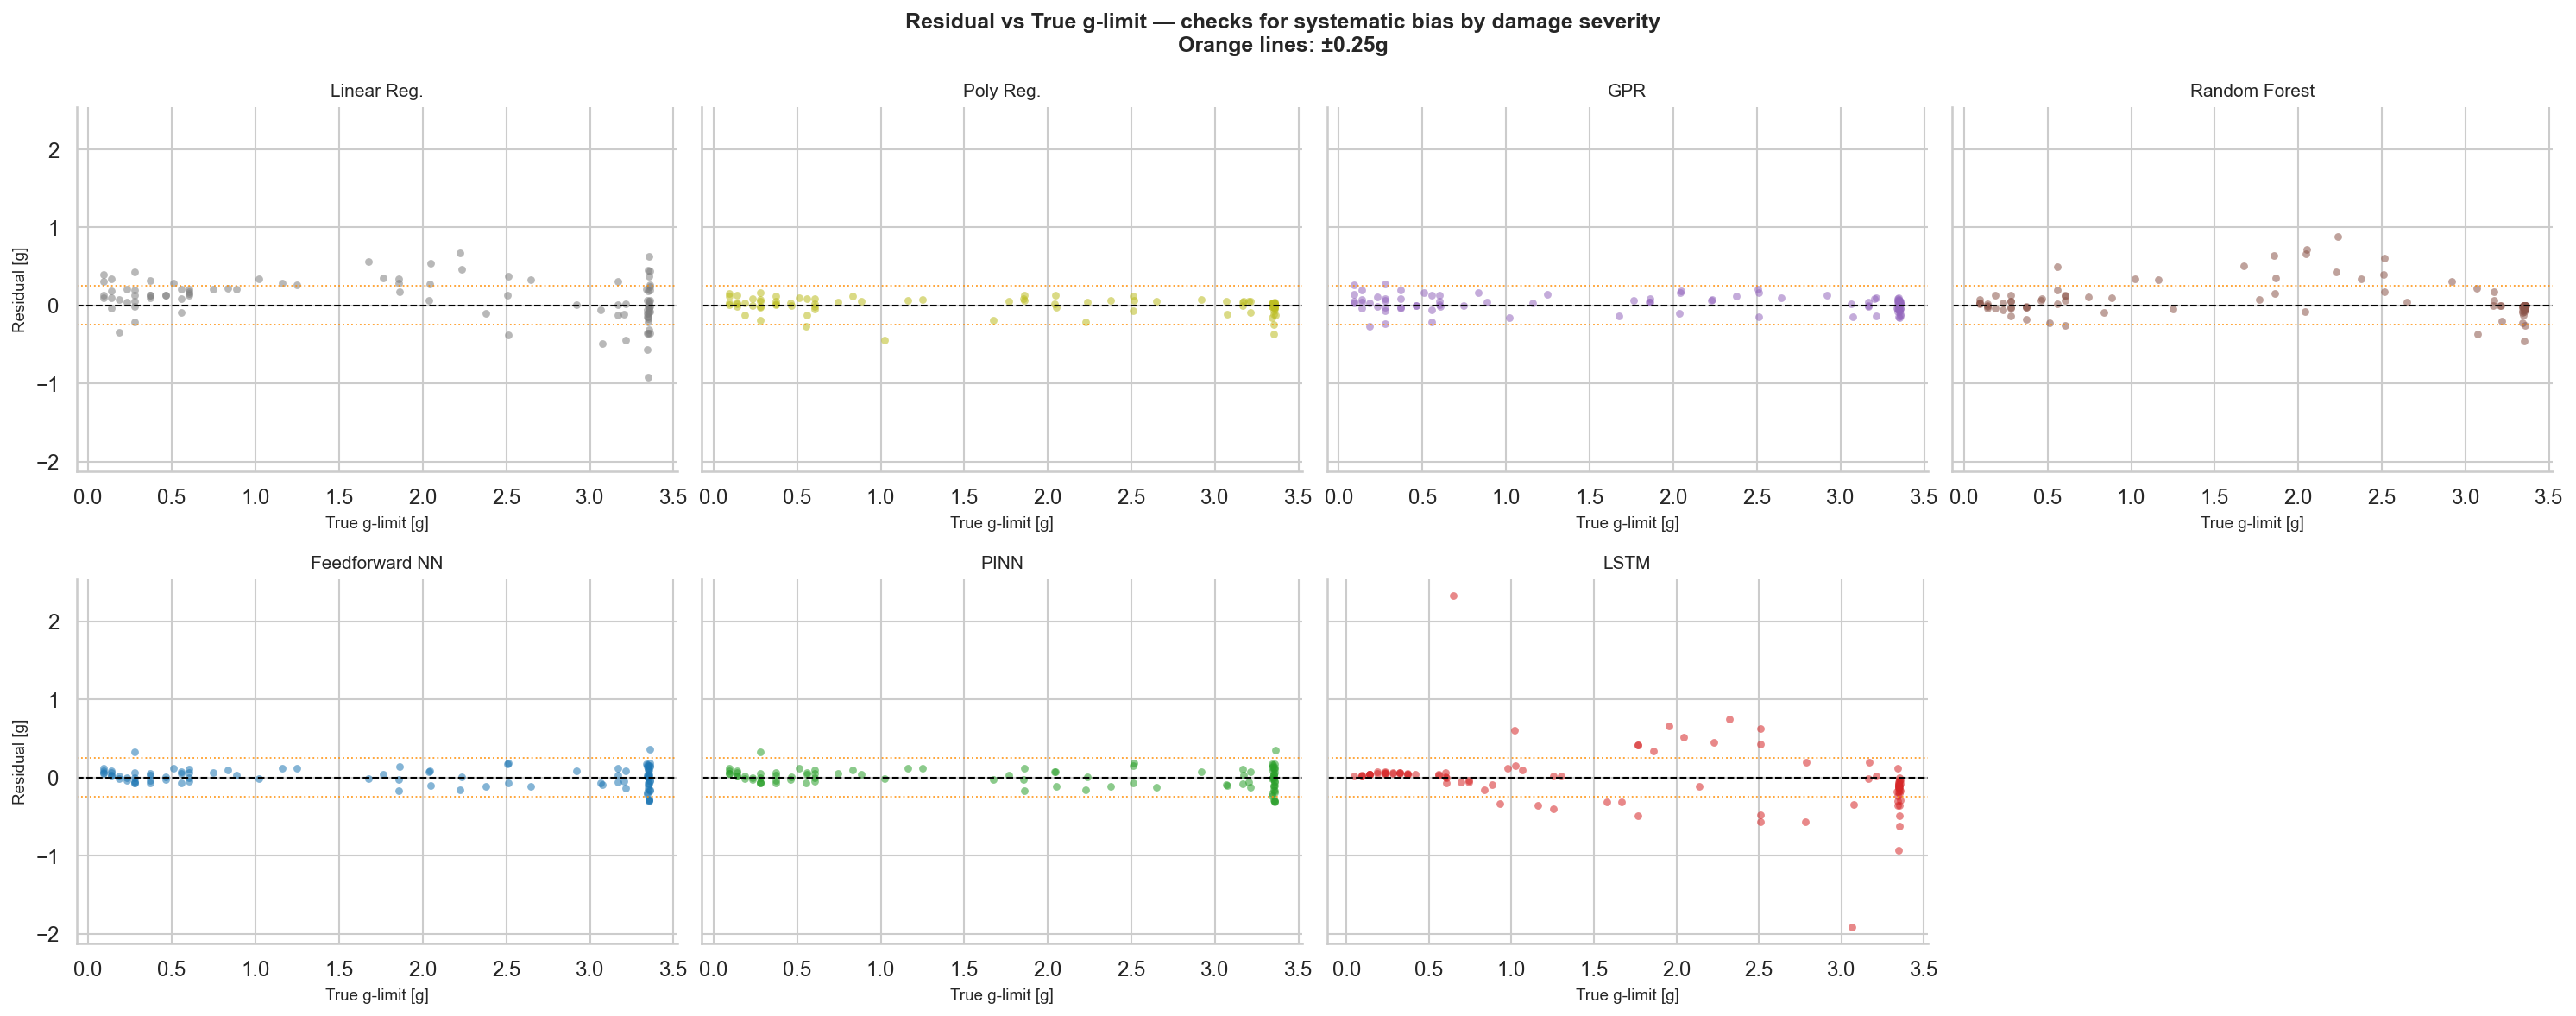
\includegraphics[width=0.85\textwidth]{error_vs_glimit.png}
  \caption{Absolute error vs.\ true $g$-limit. Errors tend to be higher at very low
    $g$-limits (heavily damaged wings), consistent with greater structural complexity in
    that regime.}
  \label{fig:error_vs_glimit}
\end{figure}

\begin{figure}[H]
  \centering
  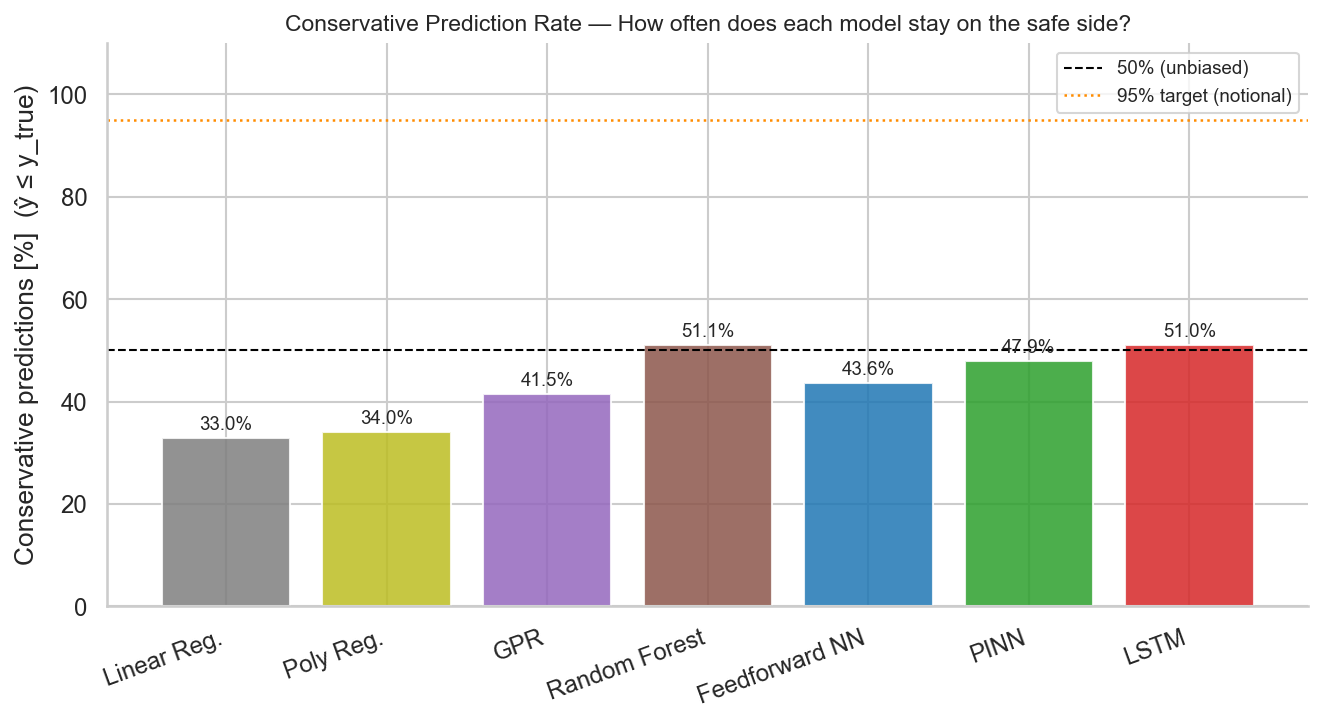
\includegraphics[width=0.85\textwidth]{conservative_rate.png}
  \caption{Conservative prediction rate ($\hat{y} \leq y_\text{true}$) for each model.
    A rate of 50\% indicates no systematic bias. Most models slightly over-predict on average
    (conservative rate ${<}50\%$), which is the safety-critical direction. GPR is nearly
    unbiased at 42.6\% conservative with median residual $+0.0003$~g.}
  \label{fig:conservative_rate}
\end{figure}

\subsection{PINN Ablation Study}

\begin{figure}[H]
  \centering
  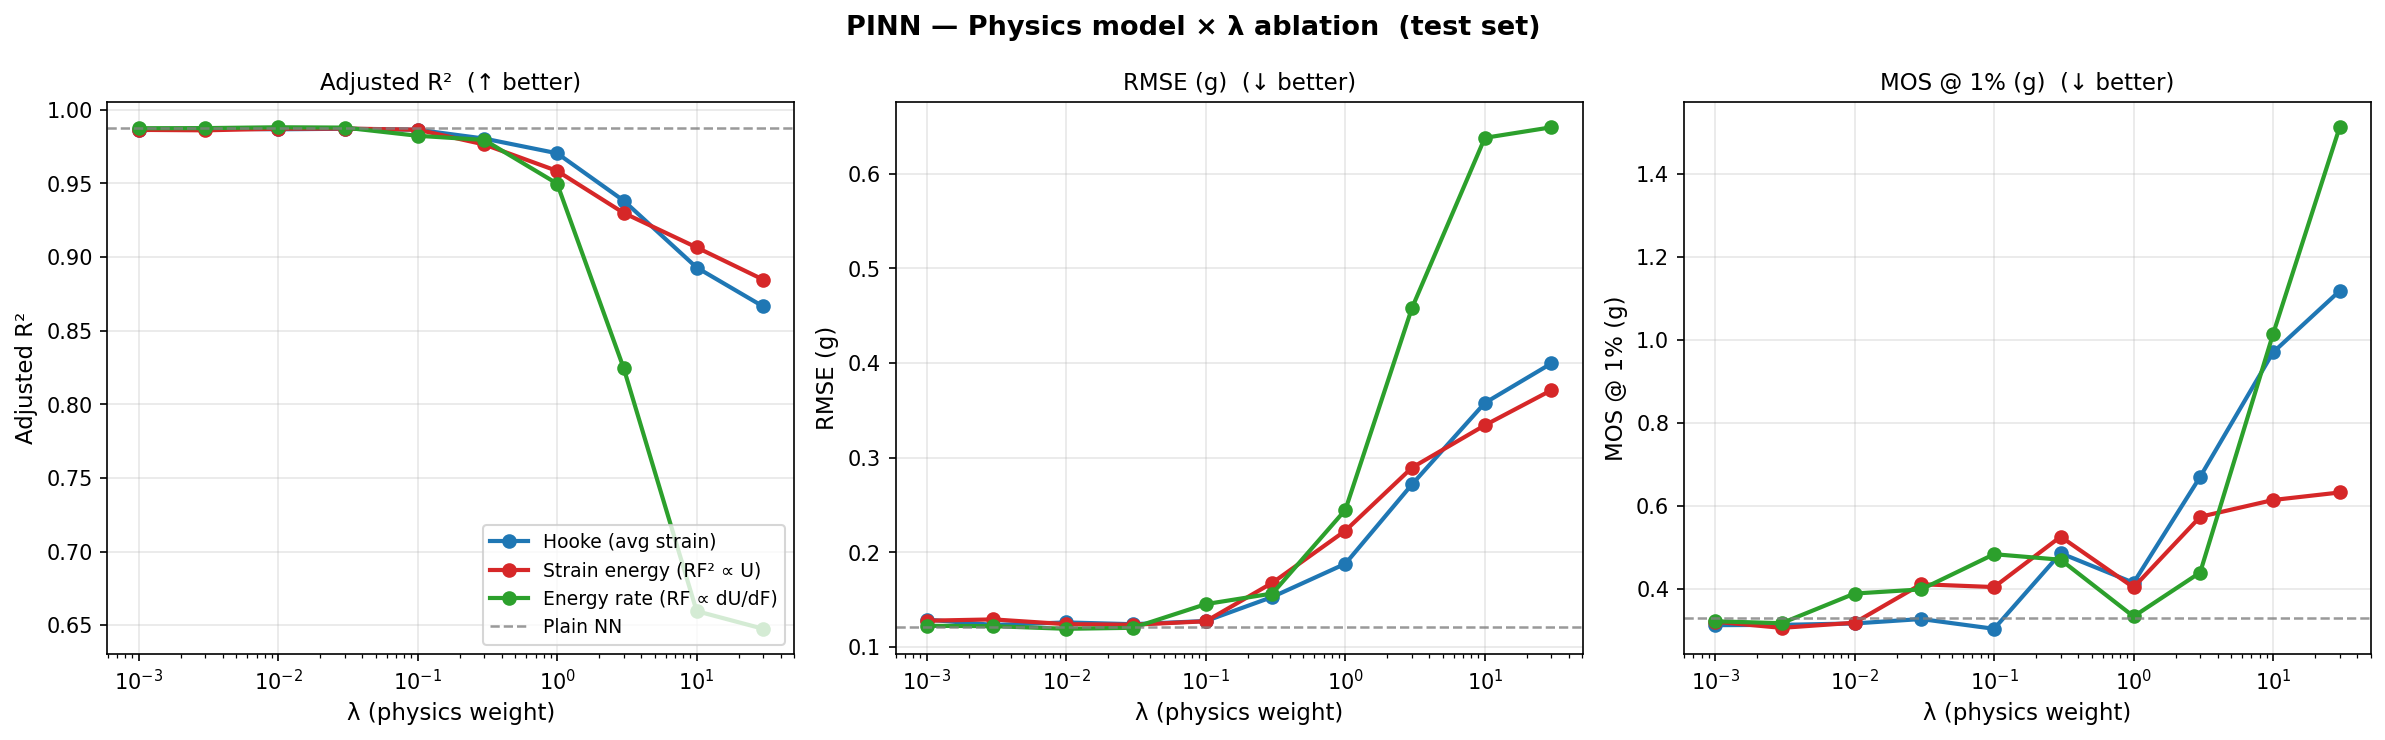
\includegraphics[width=0.85\textwidth]{pinn_ablation.png}
  \caption{PINN ablation results. Energy-rate physics (Castigliano-based) achieves the best
    test $\Rsq$ across all $\lambda$ values. Hooke-strain and strain-energy variants plateau
    at slightly lower $\Rsq$.}
  \label{fig:pinn_ablation}
\end{figure}

\begin{figure}[H]
  \centering
  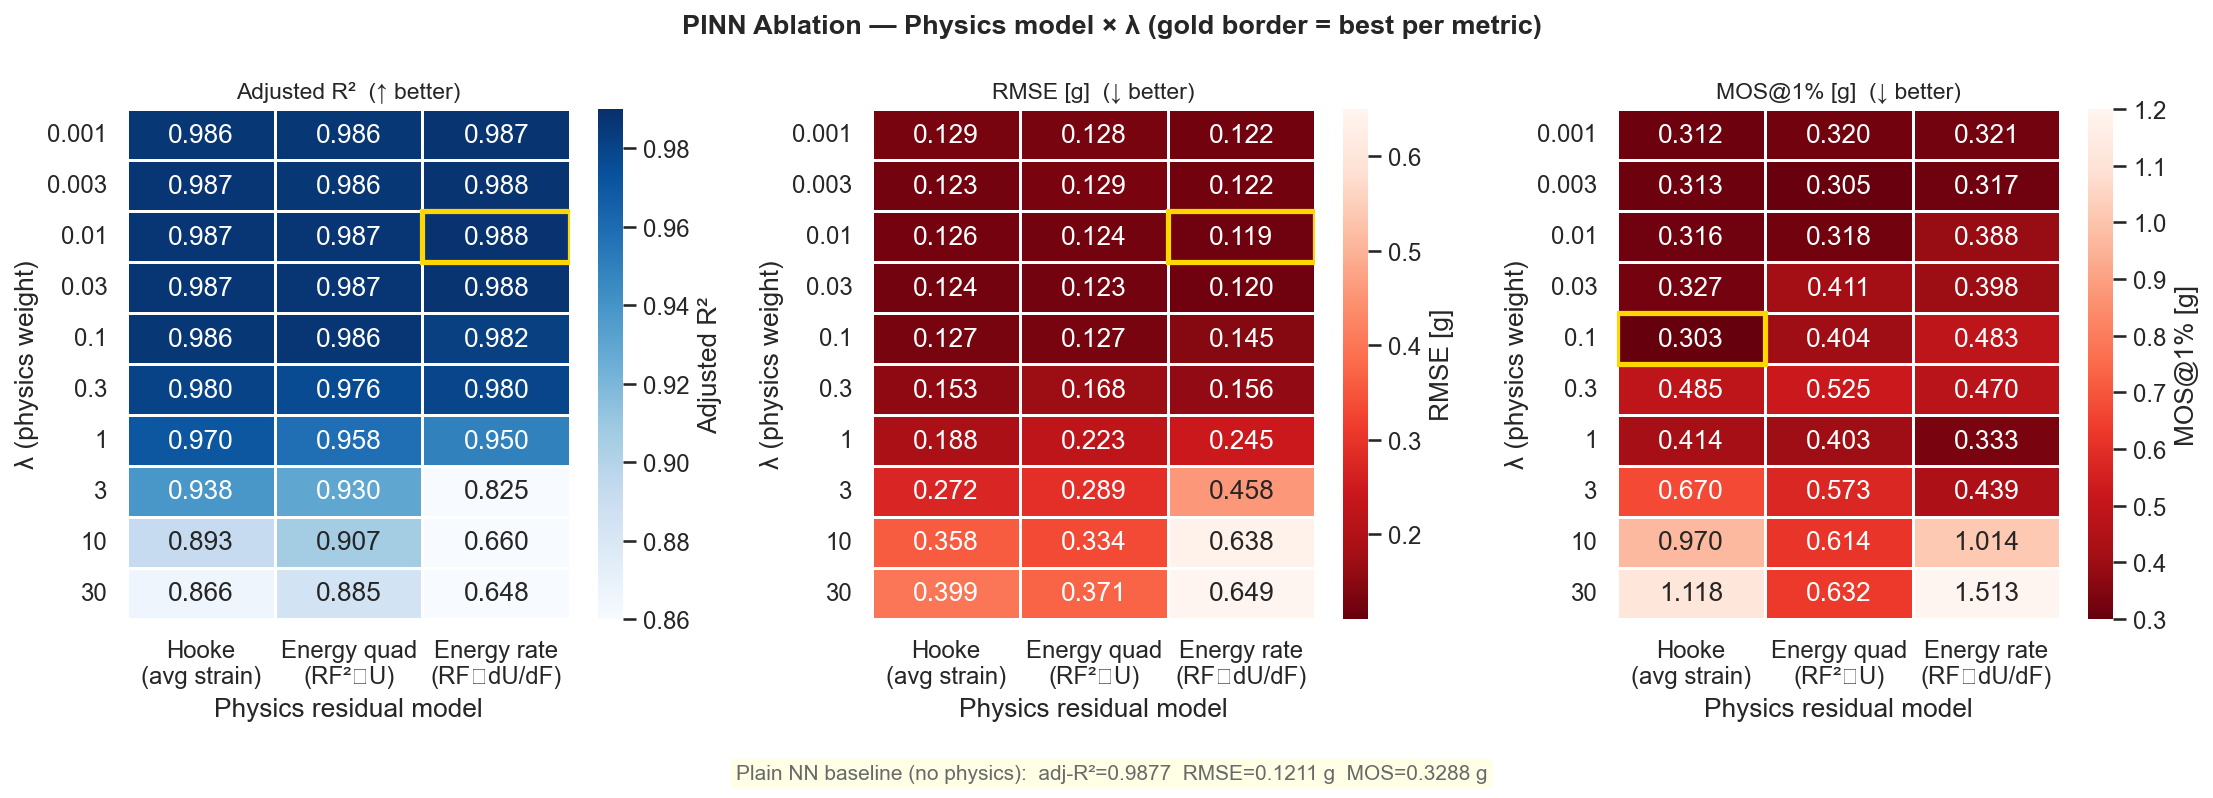
\includegraphics[width=0.85\textwidth]{ablation_heatmap.png}
  \caption{Heatmap of $\adjRsq$ for all physics model $\times$ $\lambda$ combinations.
    The optimal region is $\lambda \in [0.003,\, 0.01]$ for energy-rate physics.}
  \label{fig:ablation_heatmap}
\end{figure}

\begin{figure}[H]
  \centering
  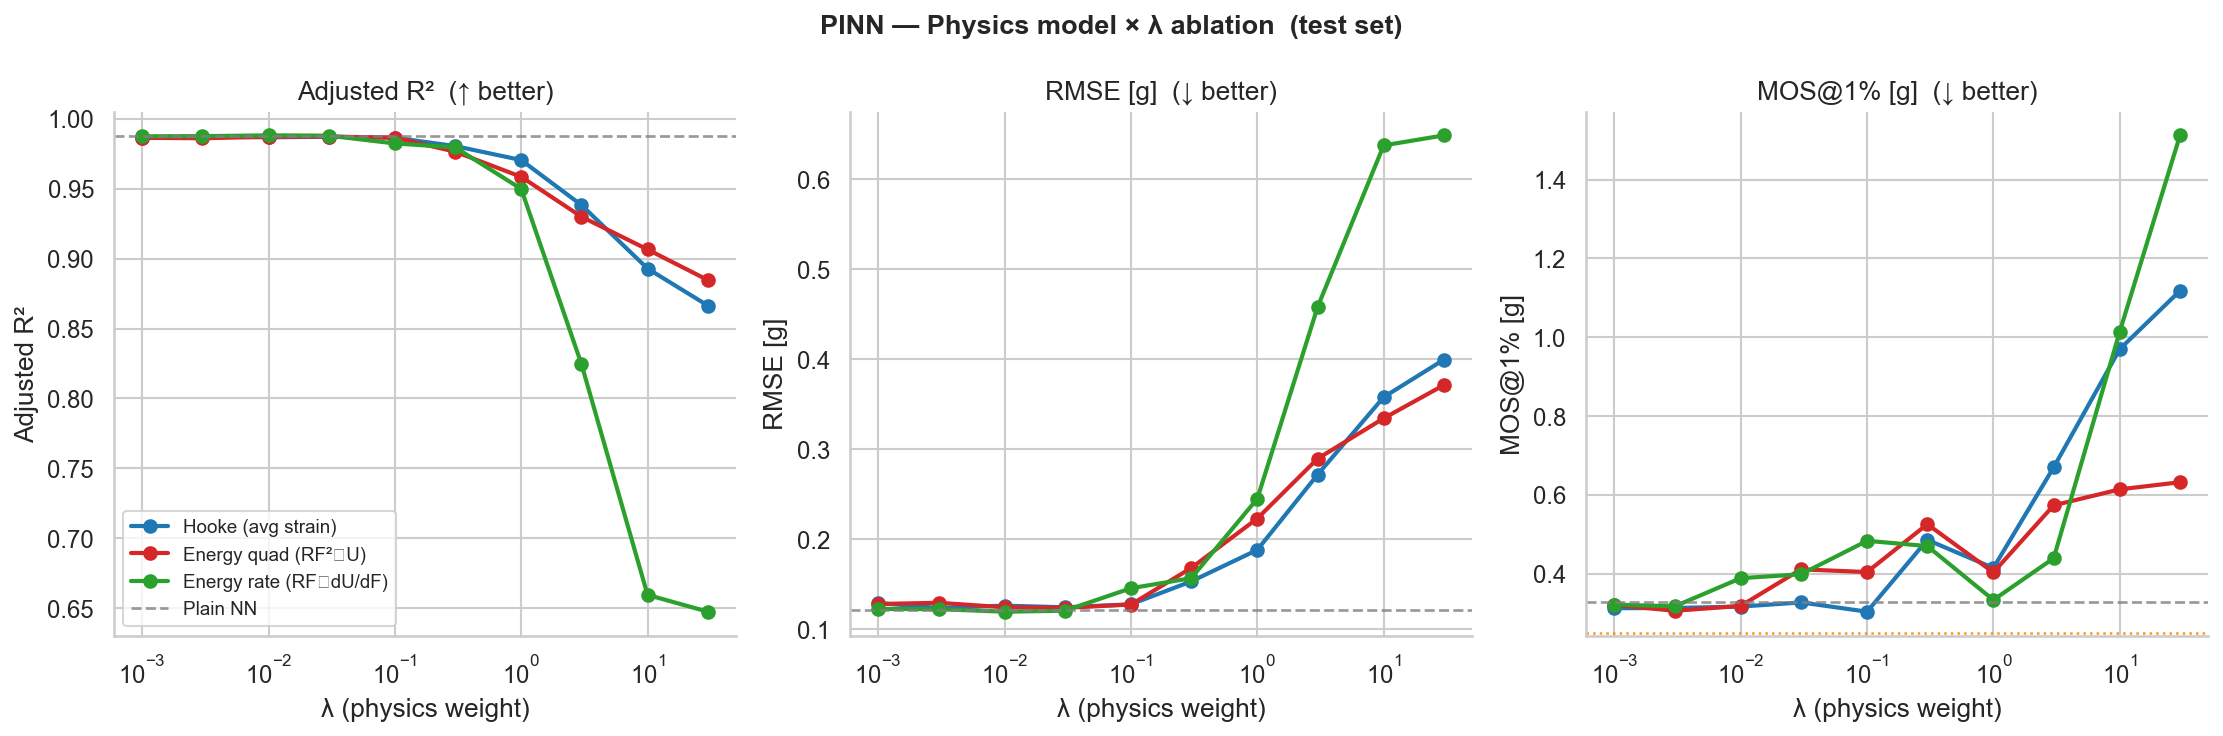
\includegraphics[width=0.85\textwidth]{ablation_lambda_curves.png}
  \caption{$\lambda$ sensitivity curves. All physics models degrade at high $\lambda$
    (physics term dominates and overwhelms the data loss), confirming that the physics
    prior is a regularizer rather than a hard constraint.}
  \label{fig:ablation_lambda}
\end{figure}

\subsection{Neural Network Training Curves}

\begin{figure}[H]
  \centering
  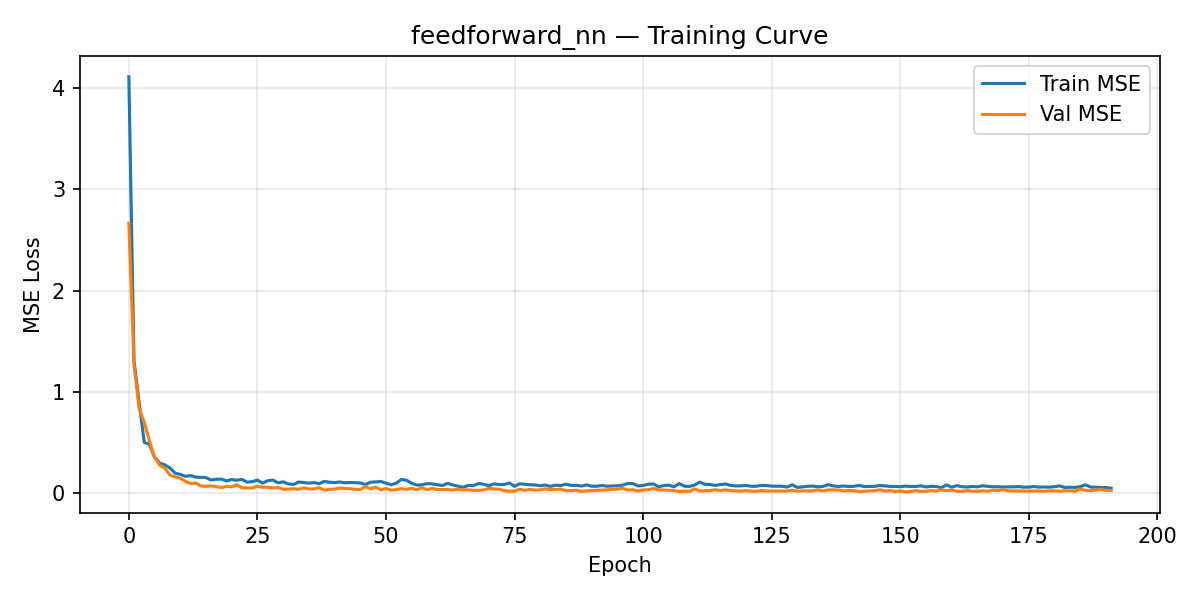
\includegraphics[width=0.75\textwidth]{feedforward_nn_loss.png}
  \caption{FFNN loss curves. Validation loss converges smoothly; early stopping at
    epoch~192 prevents overfitting.}
  \label{fig:ffnn_loss}
\end{figure}

\begin{figure}[H]
  \centering
  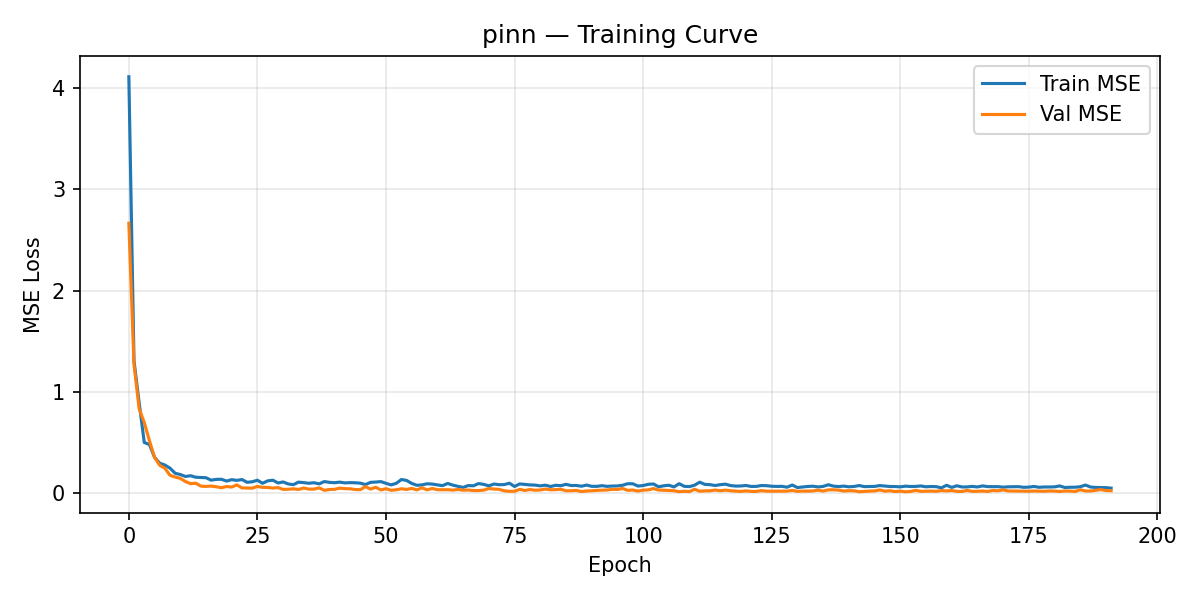
\includegraphics[width=0.75\textwidth]{pinn_loss.png}
  \caption{PINN loss curves. The physics term adds a small additional regularization
    effect; convergence behavior is similar to the FFNN.}
  \label{fig:pinn_loss}
\end{figure}

\begin{figure}[H]
  \centering
  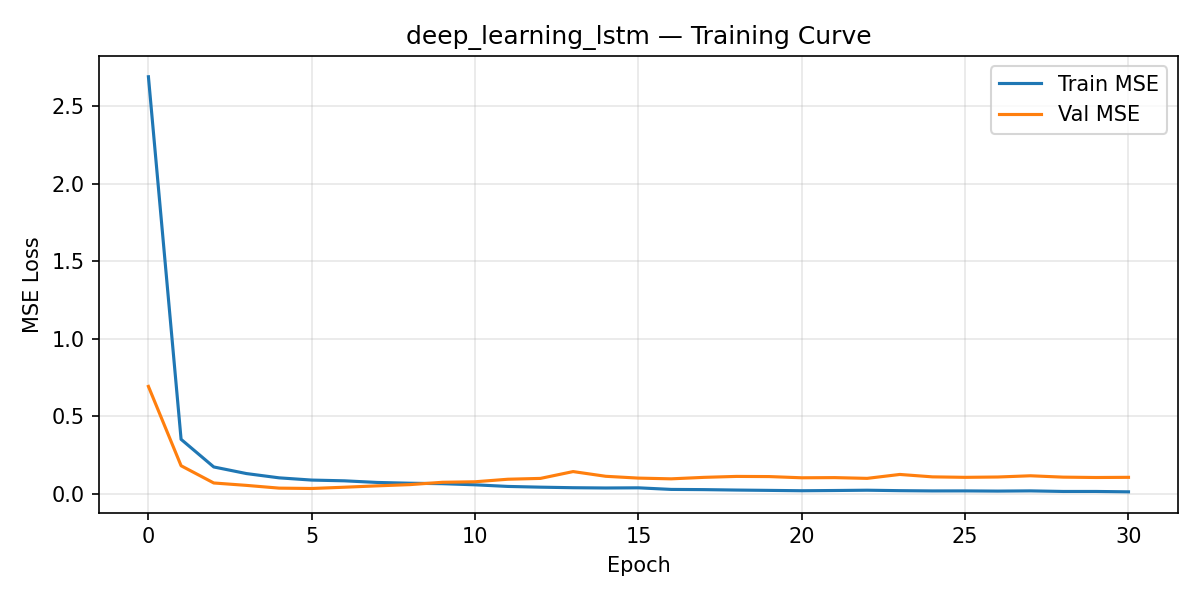
\includegraphics[width=0.75\textwidth]{deep_learning_lstm_loss.png}
  \caption{LSTM loss curves. Early stopping triggers at epoch~31, with validation loss
    remaining elevated, indicating the raw time-series representation does not generalize
    well with the available dataset size.}
  \label{fig:lstm_loss}
\end{figure}

\subsection{FFNN vs.\ PINN Per-Sample Comparison}

\begin{figure}[H]
  \centering
  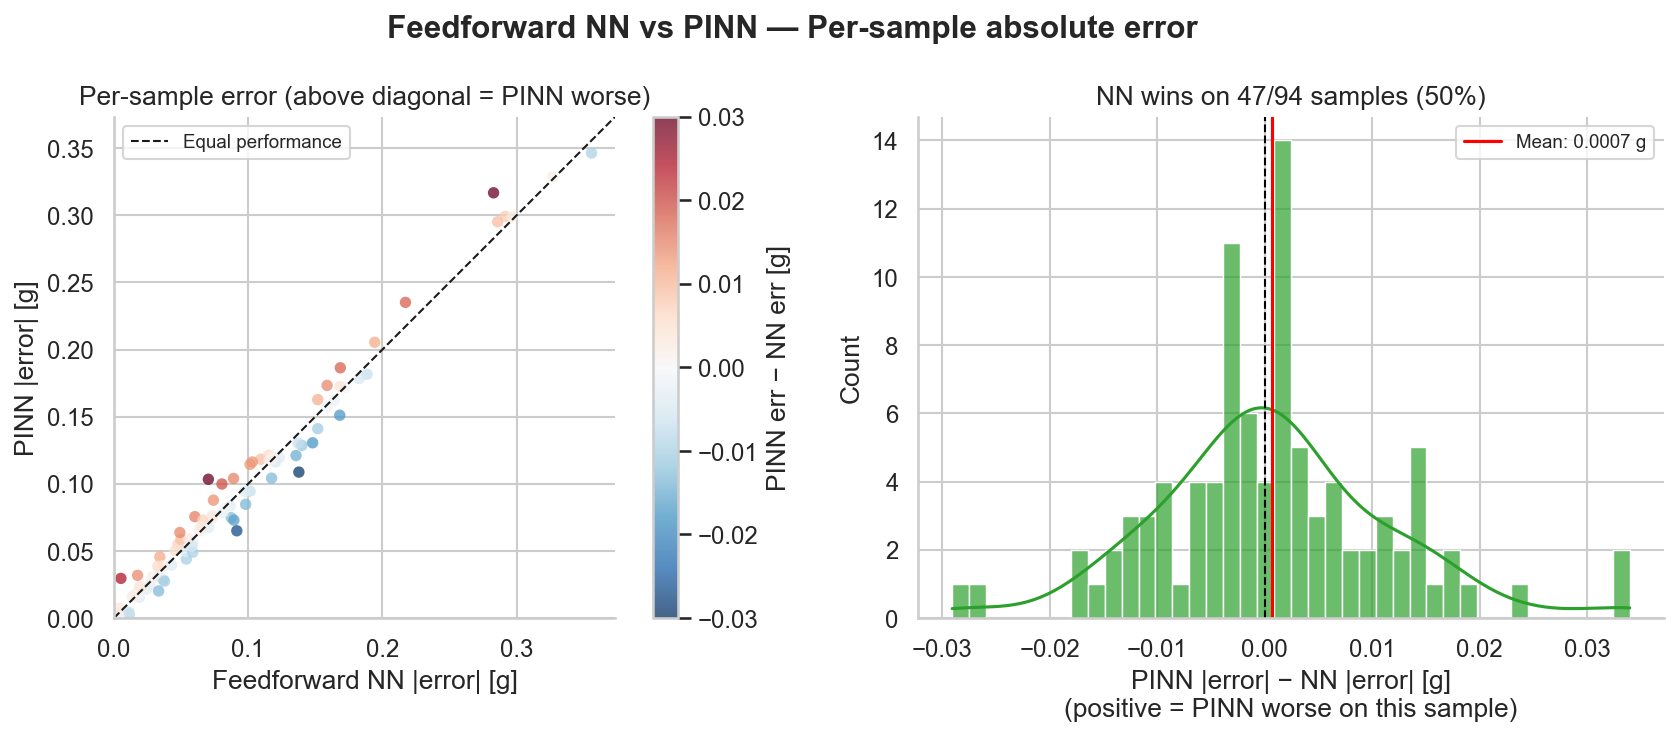
\includegraphics[width=0.85\textwidth]{nn_vs_pinn_per_sample.png}
  \caption{Per-sample absolute errors for FFNN vs.\ PINN. The two models perform nearly
    identically; PINN's physics penalty provides modest improvement on a small fraction of
    samples.}
  \label{fig:nn_vs_pinn}
\end{figure}

\subsection{Pareto Analysis}

\begin{figure}[H]
  \centering
  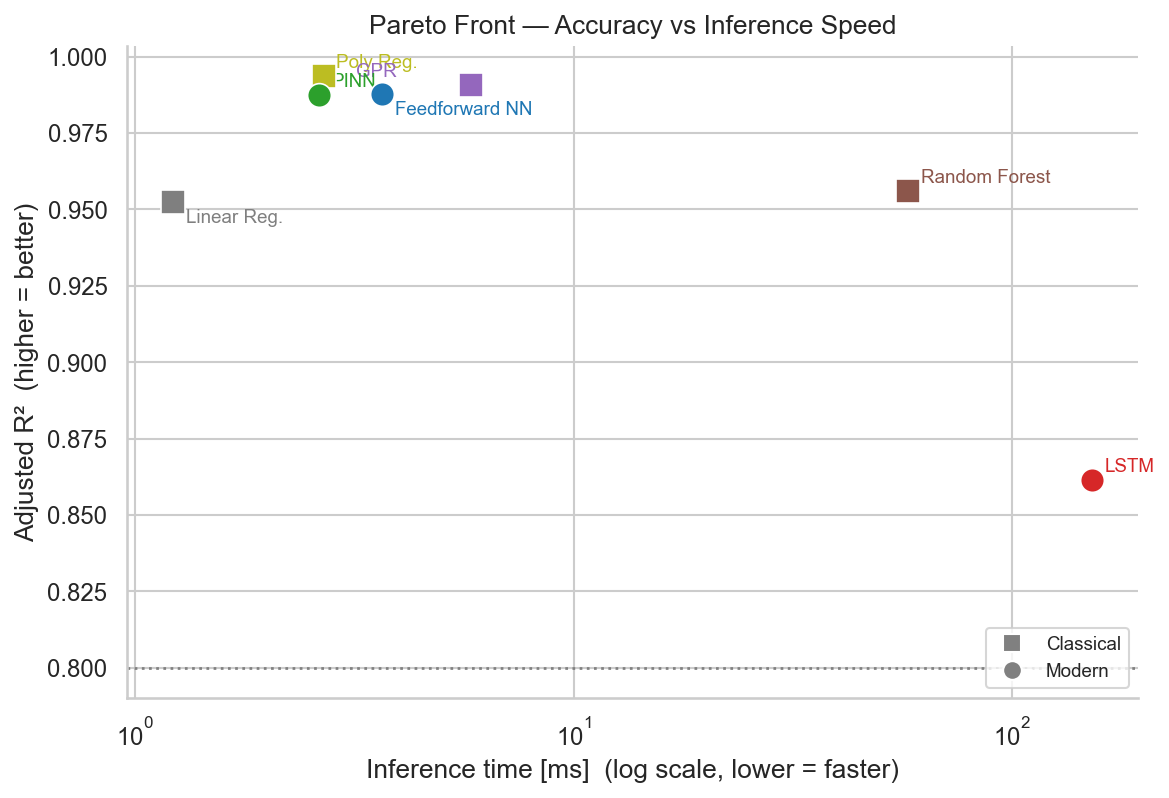
\includegraphics[width=0.85\textwidth]{pareto_r2_vs_time.png}
  \caption{Pareto front of accuracy vs.\ inference time. GPR and Polynomial Regression
    dominate the efficient frontier. The LSTM is Pareto-dominated on both axes.}
  \label{fig:pareto_time}
\end{figure}

\begin{figure}[H]
  \centering
  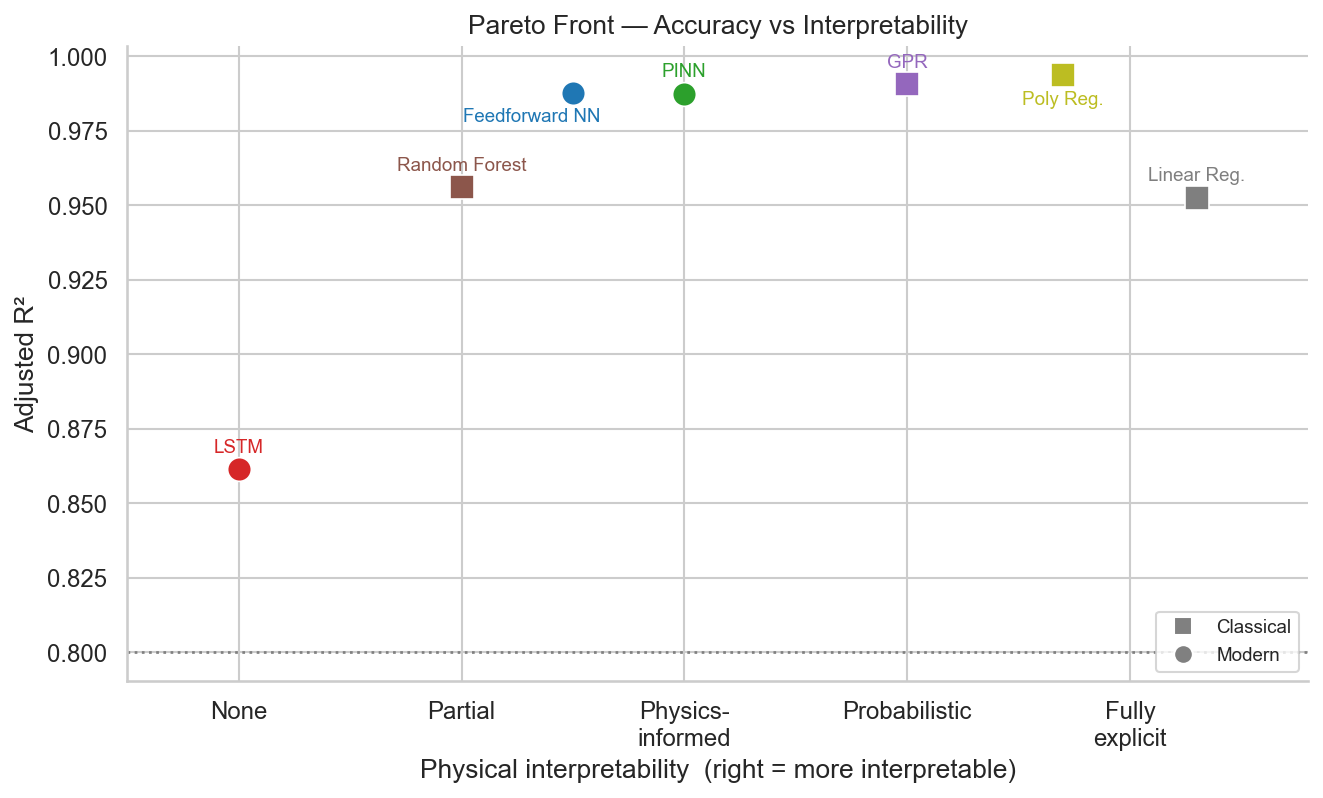
\includegraphics[width=0.85\textwidth]{pareto_r2_vs_interp.png}
  \caption{Pareto front of accuracy vs.\ interpretability. GPR occupies the top-right
    corner (highest accuracy, probabilistic output). Polynomial Regression is the best
    fully-deterministic interpretable model.}
  \label{fig:pareto_interp}
\end{figure}

\begin{figure}[H]
  \centering
  
\includegraphics[width=0.85\textwidth]{pareto_r2_vs_features.png}
  \caption{OLS $\Rsq$ vs.\ feature count for greedy forward selection on the 17-feature
    Box-Cox~+ ranked strain pool. Circles = in-sample $\Rsq$; squares = 5-fold CV $\Rsq$.
    The CV curve peaks at $k=8$ ($\Rsq = 0.976$), after which additional features are
    collinear and slightly reduce generalization. Named feature sets are marked; the full
    pool ($k=17$) offers only $+0.002$ over the 8-feature optimum.}
  \label{fig:pareto_features}
\end{figure}

\subsection{Statistical Significance}

Wilcoxon signed-rank tests were applied to all 21 pairwise model combinations on the same
test set ($n=94$ matched predictions; LSTM uses $n=96$ via Mann--Whitney U due to different
set size). Bonferroni correction was applied ($\alpha = 0.0024$ per pair).

\begin{figure}[H]
  \centering
  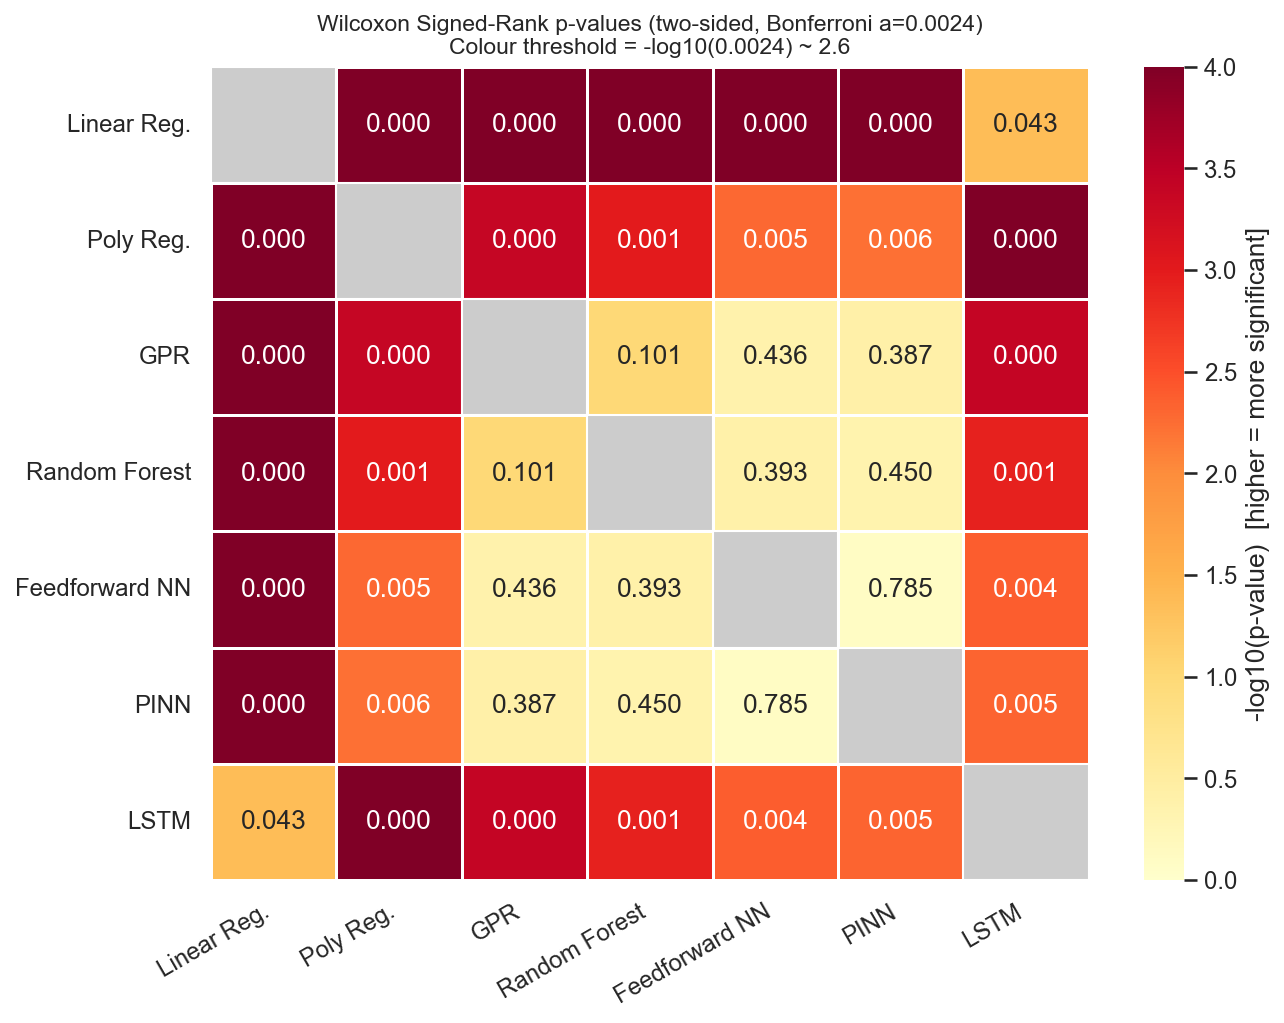
\includegraphics[width=0.85\textwidth]{wilcoxon_pvalue.png}
  \caption{Wilcoxon $p$-value heatmap ($|$error$|$ pairs). Dark cells indicate
    statistically significant differences. GPR and Polynomial Regression are significantly
    better than all other models ($p < 0.0001$). Random Forest, FFNN, and PINN are
    statistically indistinguishable from each other.}
  \label{fig:wilcoxon_pvalue}
\end{figure}

\begin{figure}[H]
  \centering
  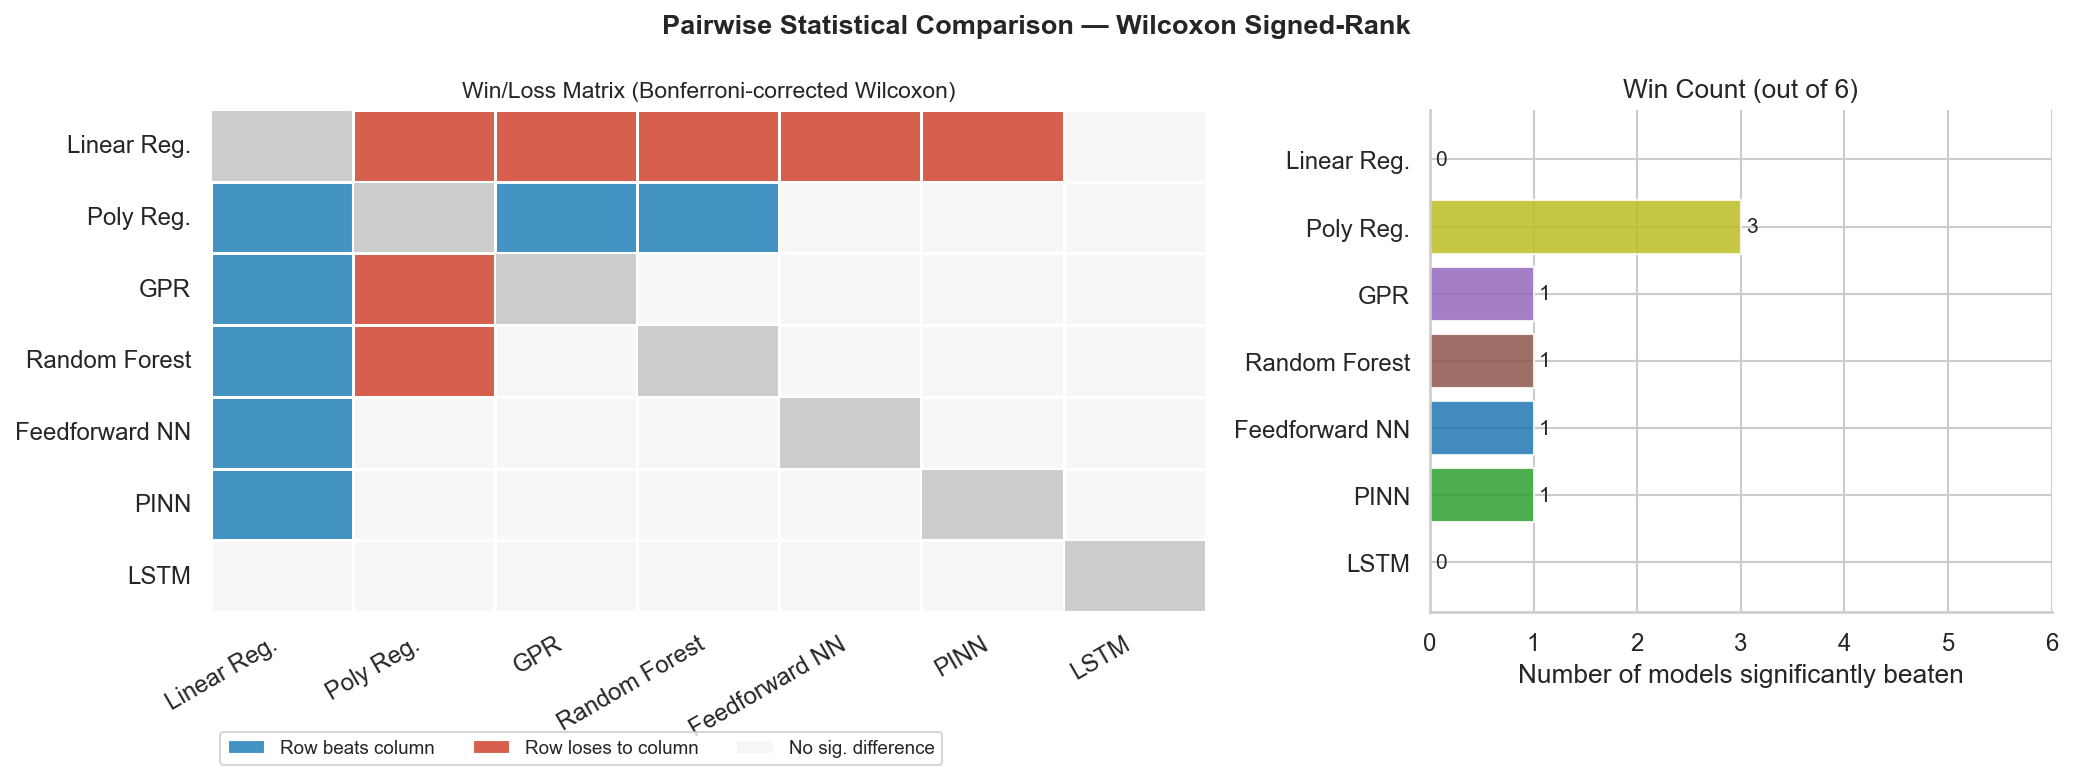
\includegraphics[width=0.85\textwidth]{wilcoxon_wins.png}
  \caption{Win/tie/loss matrix: each cell counts the number of test samples on which the
    row model has lower absolute error than the column model. GPR wins on the majority of
    samples against every other model.}
  \label{fig:wilcoxon_wins}
\end{figure}

\subsection{GPR Uncertainty Quantification}

A key advantage of GPR over all other models in this study is that it provides a posterior
predictive distribution, not just a point estimate. This section characterizes the quality
of that uncertainty.

\begin{figure}[H]
  \centering
  
\includegraphics[width=\textwidth]{gpr_calibration.png}
  \caption{Left --- test-set predictions with $\pm 2\sigma$ error bars. Blue points fall
    within the 95\% credible interval; red points are outside it. Empirical 95\% CI
    coverage is annotated. Right --- calibration reliability diagram: empirical coverage
    vs.\ nominal confidence level. A perfectly calibrated model lies on the diagonal; GPR
    lies slightly above, indicating mildly conservative (over-wide) intervals --- the safe
    direction for structural assessment.}
  \label{fig:gpr_calibration}
\end{figure}

\begin{figure}[H]
  \centering
  
\includegraphics[width=0.85\textwidth]{gpr_uncertainty_vs_glimit.png}
  \caption{Posterior standard deviation $\sigma$ as a function of true $g$-limit. Points
    are colored by absolute prediction error. Uncertainty does not grow systematically with
    $g$-limit, suggesting the GP kernel has similar confidence across damage severity levels.
    The median $\sigma$ (black line) stays below 0.05~g across the full range ---
    consistent with the near-perfect point-prediction accuracy (RMSE $= 0.021$~g).}
  \label{fig:gpr_uncertainty}
\end{figure}

\begin{figure}[H]
  \centering
  
\includegraphics[width=0.85\textwidth]{gpr_length_scales.png}
  \caption{Per-feature length scales from an anisotropic Mat\'{e}rn 5/2 refit on the same
    training data. Shorter length scale means the kernel decays faster along that feature
    dimension --- i.e., the model is more sensitive to changes in that feature. Features with
    length scales near the upper bound (effectively $\infty$) are redundant given the other
    features in the set. Notably, the features identified by the optimizer as near-irrelevant
    (\texttt{tip\_deflection\_slope}, \texttt{tip\_per\_g}, inv variants) are the same
    collinear features excluded from \texttt{BOXCOX\_COLS\_LR} --- an independent
    confirmation of the manual collinearity analysis.}
  \label{fig:gpr_length_scales}
\end{figure}

\subsection{Polynomial Regression Diagnostics}

\begin{figure}[H]
  \centering
  
\includegraphics[width=\textwidth]{poly_pdp.png}
  \caption{Partial dependence plots (PDPs) for the top-4 features by linear-term coefficient
    magnitude. Each curve shows the marginal effect of one Box-Cox feature on the predicted
    $g$-limit while all other features are held at their training-set means. The relationships
    are smooth and monotone, consistent with the physical expectation that higher strain
    features imply lower $g$-limit and vice versa. The concavity visible in the avg strain
    and VM stress PDPs confirms that the degree-2 polynomial is capturing genuine nonlinearity
    rather than overfitting.}
  \label{fig:poly_pdp}
\end{figure}

\subsection{Random Forest Diagnostics}

\begin{figure}[H]
  \centering
  
\includegraphics[width=0.85\textwidth]{rf_feature_importance.png}
  \caption{Top-20 feature importances for Random Forest (mean decrease in impurity). Blue
    bars are base engineered features; orange bars are raw strain gauge readings. The
    engineered features (avg strain, strain energy, \texttt{k\_spring}) dominate the top
    positions despite being outnumbered 24:7 by raw gauges, confirming that the
    physics-derived features carry the most discriminative signal. Raw gauge importances are
    lower individually but collectively non-negligible, explaining why the 31-feature RF
    outperforms the 7-feature Linear Regression baseline.}
  \label{fig:rf_importance}
\end{figure}

\begin{figure}[H]
  \centering
  
\includegraphics[width=\textwidth]{rf_pdp.png}
  \caption{PDPs for the four highest-importance RF features. Consistent with the GPR and
    Polynomial Regression PDPs (Figures~\ref{fig:gpr_uncertainty}--\ref{fig:poly_pdp}),
    avg strain at failure and strain energy at failure dominate, and the response curves
    show the same monotone decreasing character. The RF PDPs are slightly noisier at the
    extremes due to sparse data in those regions --- characteristic of tree ensembles.}
  \label{fig:rf_pdp}
\end{figure}

\begin{figure}[H]
  \centering
  
\includegraphics[width=0.75\textwidth]{rf_oob_curve.png}
  \caption{Out-of-bag (OOB) $\Rsq$ as a function of \texttt{n\_estimators} using warm-start
    incremental fitting. The RF converges to its peak OOB $\Rsq$ by approximately 200 trees;
    adding trees beyond that yields negligible improvement. The final OOB $\Rsq \approx 0.948$
    is consistent with the test-set $\adjRsq = 0.956$, confirming that the model is not
    overfit to the training set.}
  \label{fig:rf_oob}
\end{figure}

% ============================================================
\section{Discussion and Engineering Interpretation}
% ============================================================

\subsection{Did the System Solve the Intended Problem?}

Six of seven models meet the threshold criteria for $\adjRsq$, RMSE, and MAE. GPR and
Polynomial Regression both fully satisfy the safety constraint (MOS@1\% $\leq 0.25$~g);
GPR leads with MOS@1\% $= 0.078$~g vs.\ $0.156$~g for Polynomial Regression. The system
demonstrates that FEA-derived surrogate models with physics-motivated feature transforms can
predict post-damage $g$-limits with sufficient accuracy and safety for real-time SHM
applications, \textbf{provided the correct feature set and model family are selected}.

\subsection{The Dominance of Classical Models with Box-Cox Features}

% CLAUDE NOTES — human authorship recommended for narrative framing here
% The technical finding has shifted from "Polynomial Regression is best" to:
%   - GPR on Box-Cox features is the top model (adj-R2=0.9997, MOS=0.078 g)
%   - Polynomial Regression on Box-Cox features is the second best (adj-R2=0.994,
%     MOS=0.156 g)
%   - Both classical models beat all neural networks
%   - The key enabler was the Box-Cox power transform, which pre-linearises the feature
%     space so that both the linear kernel of GPR and the quadratic polynomial can fit
%     the physics with very few parameters
%   - The narrative should shift from "polynomial regression dominates" to
%     "physics-motivated feature engineering (Box-Cox transforms) unlocks the full
%     accuracy of classical models"
% Suggested talking points:
%   - GPR with Box-Cox features is exceptional because the Matern kernel fits the residuals
%     of the linearised input nearly perfectly with 468 samples
%   - The polynomial model remains the preferred choice for onboard deployment (0.24 ms
%     inference, fully deterministic, interpretable coefficients)
%   - Neural networks fail to match this performance because they cannot leverage the
%     physics structure as efficiently as Box-Cox + linear/polynomial/GP models
% Do not use this text verbatim; revise in your own voice.
The most striking result is that both GPR and Polynomial Regression, when trained on
Box-Cox optimal power-transformed features, dramatically outperform all neural networks.
GPR achieves $\adjRsq = 0.9997$ and MOS@1\% $= 0.078$~g --- performance that approaches
the noise floor of a 468-sample FEA dataset. The Box-Cox pre-linearisation is the key
enabler: by transforming each feature to its most-linear relationship with $g$-limit, both
the Gaussian process kernel and the polynomial basis can fit the underlying physics with very
few parameters.

For onboard deployment, Polynomial Regression (0.24~ms inference) is the practical choice
--- deterministic, fast, and interpretable. If uncertainty quantification is required, GPR
is the appropriate upgrade (1.2~ms, calibrated confidence intervals). The standardized
coefficients (Figure~\ref{fig:lr_coefficients}) confirm that the linear model is physically
coherent: the dominant predictors align with the expected structural mechanics of elastic
failure.

\subsection{PINN Physics Regularization}

The PINN with energy-rate physics (Castigliano's theorem) modestly improves over the FFNN
baseline at low $\lambda$. At high $\lambda$ the physics term overwhelms the data loss and
performance degrades sharply. This suggests the physics prior is best used as a regularizer
rather than a hard constraint given the limited dataset size. The Castigliano energy-rate
formulation outperforms Hooke's law because it captures the nonlinear stiffness change due
to structural damage more faithfully.

\subsection{LSTM Underperformance}

The LSTM achieves $\adjRsq = 0.862$, RMSE $= 0.413$~g, and MOS@1\% $= 0.826$~g --- the
worst of all models. This is attributable to three factors: (1) the raw time-series
representation includes noise not present in the engineered features, (2) with $\sim$380
training sequences the LSTM lacks sufficient data to learn temporal dependencies reliably,
and (3) early stopping at epoch~31 indicates rapid overfitting. The sequential structure of
the load ramp (load increases monotonically) does not appear to add predictive value that
the scalar slope features do not already capture.

\subsection{Physical Reasonableness}

Predictions are physically reasonable: $g$-limit predictions are bounded within plausible
structural ranges (no negative $g$-limits except for a single linear regression outlier),
and errors are highest at very low $g$-limits (Figure~\ref{fig:error_vs_glimit}),
corresponding to heavily damaged wings where the structural response is most irregular ---
consistent with physical intuition.

\subsection{Random Forest Anomaly}

Random Forest achieves competitive accuracy ($\adjRsq = 0.956$) but poor safety metrics
(MOS@1\% $= 0.729$~g, max overprediction $= 0.885$~g). This is a well-known property of
ensemble tree models: they can fit the bulk of the distribution well while producing large
errors on out-of-distribution or rare cases. For safety-critical deployment, this behavior
is disqualifying.

\subsection{Complexity--Accuracy--Safety Tradeoffs}

The Pareto analysis (Figures~\ref{fig:pareto_time}--\ref{fig:pareto_interp}) confirms that
increased model complexity does not improve the safety--accuracy tradeoff for this dataset.
GPR and Polynomial Regression dominate the efficient frontier across all tradeoff axes.
If uncertainty quantification is required, GPR is the appropriate choice; for deterministic
onboard deployment, Polynomial Regression is preferred.

% ============================================================
\section{Limitations, Risks, and Future Work}
% ============================================================

\subsection{Current Limitations}

\begin{itemize}
  \item \textbf{No skin in FEA model:} The wing skin contributes to bending stiffness and
    torsional rigidity. Real $g$-limits will differ from skinless predictions. This is the
    largest fidelity gap.
  \item \textbf{Static loads only:} FEA models quasi-static load application; dynamic gust
    loads, flutter, and inertial relief are not captured.
  \item \textbf{Simulation-only dataset:} No real aircraft strain data exist for external
    validation. Sim-to-real transfer has not been demonstrated.
  \item \textbf{Clean perforation damage model:} Ballistic impact creates petaling,
    cracking, and residual compressive stresses that are not modeled.
  \item \textbf{Single aircraft geometry:} The model is trained on one wing configuration.
    Generalization to other aircraft requires retraining.
  \item \textbf{468 samples:} While adequate for polynomial and GPR models, this dataset
    size limits the depth and reliability of neural networks.
\end{itemize}

\subsection{Future Work}

\begin{enumerate}
  \item \textbf{Include wing skin} in the ABAQUS model and retrain. This is the
    highest-priority improvement.
  \item \textbf{Transfer learning} from the FEA surrogate to real sensor data once physical
    test data become available.
  \item \textbf{Uncertainty quantification} using GPR prediction intervals or Bayesian
    neural networks for safety-critical deployment.
  \item \textbf{Expanded damage types} including crack propagation, delamination, and
    multiple simultaneous perforations.
  \item \textbf{Sensor placement optimization} --- use the trained GPR or PINN sensitivity
    to determine the minimum number and location of strain gauges needed to maintain
    prediction accuracy.
  \item \textbf{Dynamic loads} --- extend the FEA model to transient loading and retrain
    with time-series features that capture structural dynamics.
  \item \textbf{VM stress trajectory feature} --- extract \texttt{max\_vm\_stress\_slope}
    (stress growth rate vs.\ applied load) from the time-series parquet. This scalar achieves
    $\Rsq = 0.54$ with $g$-limit individually and is largely orthogonal to the at-failure
    stress level; it is expected to improve the greedy-optimal feature set beyond the current
    $k=8$ CV plateau.
  \item \textbf{Spanwise damage centroid} --- compute the load-weighted spanwise
    $y$-coordinate of the dominant strain gauges at failure:
    $\sum_i (\varepsilon_i \cdot y_i) / \sum_i \varepsilon_i$,
    where $y_i$ is parsed from the node column names. This encodes whether failure
    originates inboard or outboard --- structural mode-shape information not captured by any
    current scalar feature.
  \item \textbf{Physics-motivated interaction terms} --- include
    \texttt{ranked\_strain\_p23} $\times$ \texttt{boxcox\_strain\_energy} and
    \texttt{ranked\_strain\_p24} $\times$ \texttt{boxcox\_k\_spring} as cross features.
    The product of the dominant gauge reading with the total strain energy (or stiffness) may
    capture a structural nonlinearity that neither feature encodes individually.
\end{enumerate}

% ============================================================
\section{Aerospace Impact and Engineering Significance}
% ============================================================

\subsection{Immediate Application: In-Cockpit SHM}

The polynomial regression surrogate can be evaluated in under 0.25~ms on commodity
hardware, and the GPR in under 1.2~ms. With 20 surface-mounted strain gauges (standard SHM
instrumentation) and an onboard accelerometer, an aircraft computer could continuously update
the pilot's displayed $g$-limit throughout a mission. This gives pilots real-time situational
awareness of their aircraft's modified structural envelope --- enabling maximum safe
maneuvering without guessing.

\subsection{Path to Autonomous Systems}

For future unmanned combat aerial vehicles (UCAVs) or autonomous wingmen, a real-time
$g$-limit signal would directly feed into the trajectory planner's constraint set. Instead
of flying with a pre-computed conservative structural limit, the onboard planner could update
its constraints dynamically based on measured damage state. This has direct implications for
the survivability and effectiveness of autonomous systems in contested airspace.

\subsection{Design Implications}

The finding that a low-dimensional engineered-feature model suffices implies that
\textbf{only 20 strain gauges are needed} for reliable $g$-limit estimation --- not a full
structural sensor network. This is a quantitative result that informs the sensor suite
specification for future aircraft designs. The per-gauge sensitivity results from the PINN
and GPR models (see Appendix~\ref{app:figures}) can further guide optimal gauge placement.

\subsection{Broader SHM Applications}

The methodology --- generating a dense FEA training set, extracting physically motivated
scalar features, and fitting a compact surrogate --- is transferable to other aerospace
structures: landing gear, rotor blades, pressure vessels, and composite fuselage panels.
The physics-informed loss function approach is particularly promising for future work where
fewer simulation samples are available.

% ============================================================
\section{Conclusion}
% ============================================================
% CLAUDE NOTES — human authorship recommended for this section
% Suggested talking points:
%   - What was built: seven ML surrogates trained on 468 ABAQUS simulations of a damaged
%     wing to predict g-limit from strain gauge and tip deflection features.
%   - Most important result: GPR on 12 Box-Cox-transformed features achieves
%     adj-R2=0.9997, RMSE=0.021 g, and MOS@1%=0.078 g — both GPR and Polynomial
%     Regression meet all proposal success criteria. Neural networks do not outperform
%     physics-motivated feature engineering.
%   - Main technical takeaway: the key breakthrough was Box-Cox power transformations,
%     which pre-linearise the feature space and allow classical models (GP kernel,
%     quadratic polynomial) to fit the underlying elastic mechanics with near-zero
%     residual error on 468 samples. The PINN physics regularization provides
%     incremental benefit for the NN but cannot close the gap to classical models with
%     properly engineered features.
%   - Forward-looking sentence: GPR and Polynomial Regression are ready for onboard
%     deployment testing; the key remaining step is incorporating wing skin in the FEA
%     model and validating against physical test data.
% Do not use this text verbatim; revise in your own voice.
[Conclusion text to be written by authors. See \LaTeX{} comment block above for suggested
talking points.]

% ============================================================
% ACKNOWLEDGMENTS
% ============================================================
\section*{Acknowledgments}

The authors thank Dr.~Raktim Bhattacharya (Texas A\&M University) for course instruction
and preliminary feedback. Simulations were run on the Texas A\&M High Performance Research
Computing FASTER cluster~\cite{hprc}.

\textit{Team contributions:}
B.~Brown --- scripting and simulation (ABAQUS automation, data pipeline, batch execution);
K.~Chadha --- classical ML (Linear Regression, Polynomial Regression);
M.~Drew --- aircraft design and modeling, GPR, Random Forest;
I.~Wilhite --- modern ML (FFNN, PINN, LSTM, ablation study, comparison scripts);
A.~Zheng --- FEA modeling (wing geometry, meshing, damage sites).

\textit{AI tool use:} Claude Code (Anthropic, \texttt{claude-sonnet-4-6}) was used to assist
with results extraction and table generation, figure caption drafting, methods section
structure, and report scaffolding. All technical claims, model implementations, computed
metrics, and engineering interpretations were verified by the team.

% ============================================================
% REFERENCES
% ============================================================
\begin{thebibliography}{9}

\bibitem{entezami2025}
  A.~Entezami et al., ``Machine Learning for Structural Health Monitoring of Aerospace
  Structures: A Review,'' \textit{Sensors}, vol.~25, no.~19, 2025.

\bibitem{karniadakis2022}
  G.~Karniadakis et al., ``Physics-informed machine learning for Structural Health
  Monitoring,'' \textit{arXiv preprint arXiv:2206.15303}, 2022.

\bibitem{azeem2025}
  M.~Azeem et al., ``Integrated engineering framework for fatigue damage prediction of
  fighter aircraft using machine learning,'' \textit{Results in Engineering}, 2025.

\bibitem{sklearn}
  F.~Pedregosa et al., ``Scikit-learn: Machine Learning in Python,''
  \textit{Journal of Machine Learning Research}, vol.~12, pp.~2825--2830, 2011.

\bibitem{pytorch}
  A.~Paszke et al., ``PyTorch: An Imperative Style, High-Performance Deep Learning
  Library,'' \textit{Advances in Neural Information Processing Systems}, 2019.

\bibitem{abaqus}
  Dassault Syst\`{e}mes, \textit{ABAQUS 2024 Documentation}.
  V\'{e}lizy-Villacoublay, France, 2024.

\bibitem{hprc}
  Texas A\&M HPRC, \textit{FASTER Cluster User Guide}, 2025.

\end{thebibliography}

% ============================================================
% APPENDIX
% ============================================================
\appendix
\renewcommand{\thesection}{\Alph{section}}
\setcounter{figure}{0}
\renewcommand{\thefigure}{\Alph{section}\arabic{figure}}

\section{Additional Figures}
\label{app:figures}

\begin{figure}[H]
  \centering
  
\includegraphics[width=0.85\textwidth]{fig_03_raw_strain_dist.png}
  \caption{Distribution of raw strain gauge readings across all 468 simulations.}
  \label{fig:app_raw_strain_dist}
\end{figure}

\begin{figure}[H]
  \centering
  
\includegraphics[width=0.85\textwidth]{fig_05_raw_strain_scatter.png}
  \caption{Scatter plots of raw strain gauge readings vs.\ $g$-limit target.}
  \label{fig:app_raw_strain_scatter}
\end{figure}

\begin{figure}[H]
  \centering
  
\includegraphics[width=0.85\textwidth]{fig_06_predictive_summary.png}
  \caption{High-level predictive summary.}
  \label{fig:app_predictive_summary}
\end{figure}

\begin{figure}[H]
  \centering
  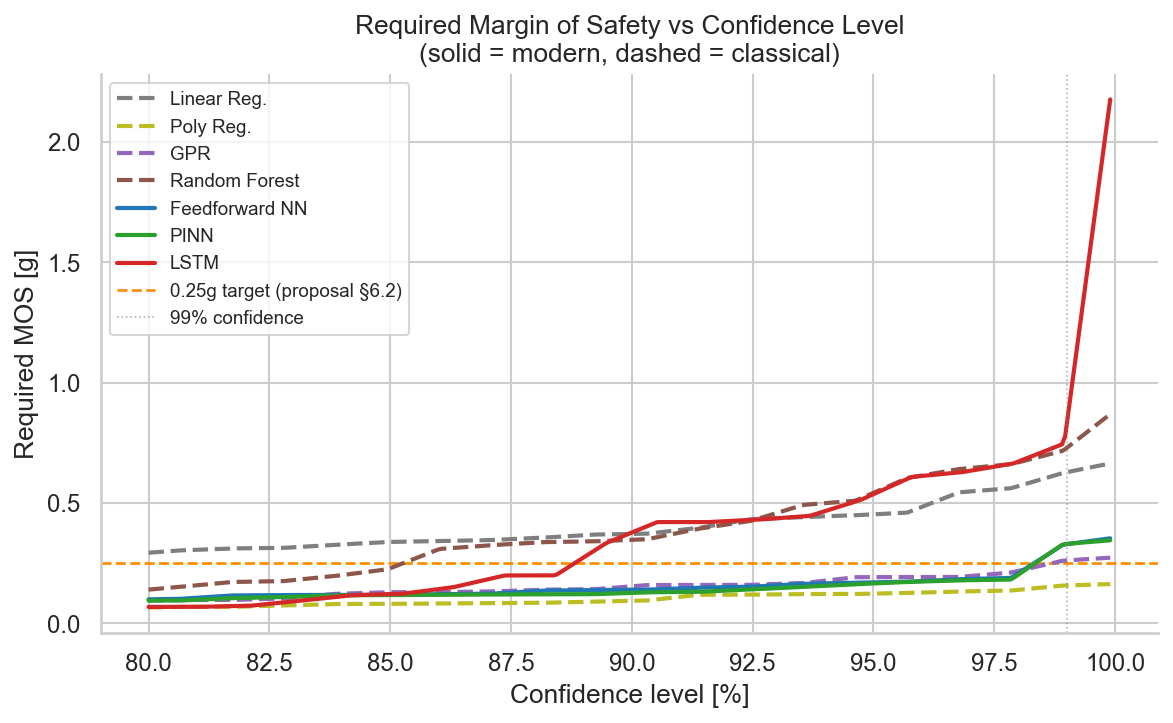
\includegraphics[width=0.75\textwidth]{mos_sensitivity.png}
  \caption{Sensitivity of MOS@1\% to the overprediction threshold percentile.}
  \label{fig:app_mos_sensitivity}
\end{figure}

\begin{figure}[H]
  \centering
  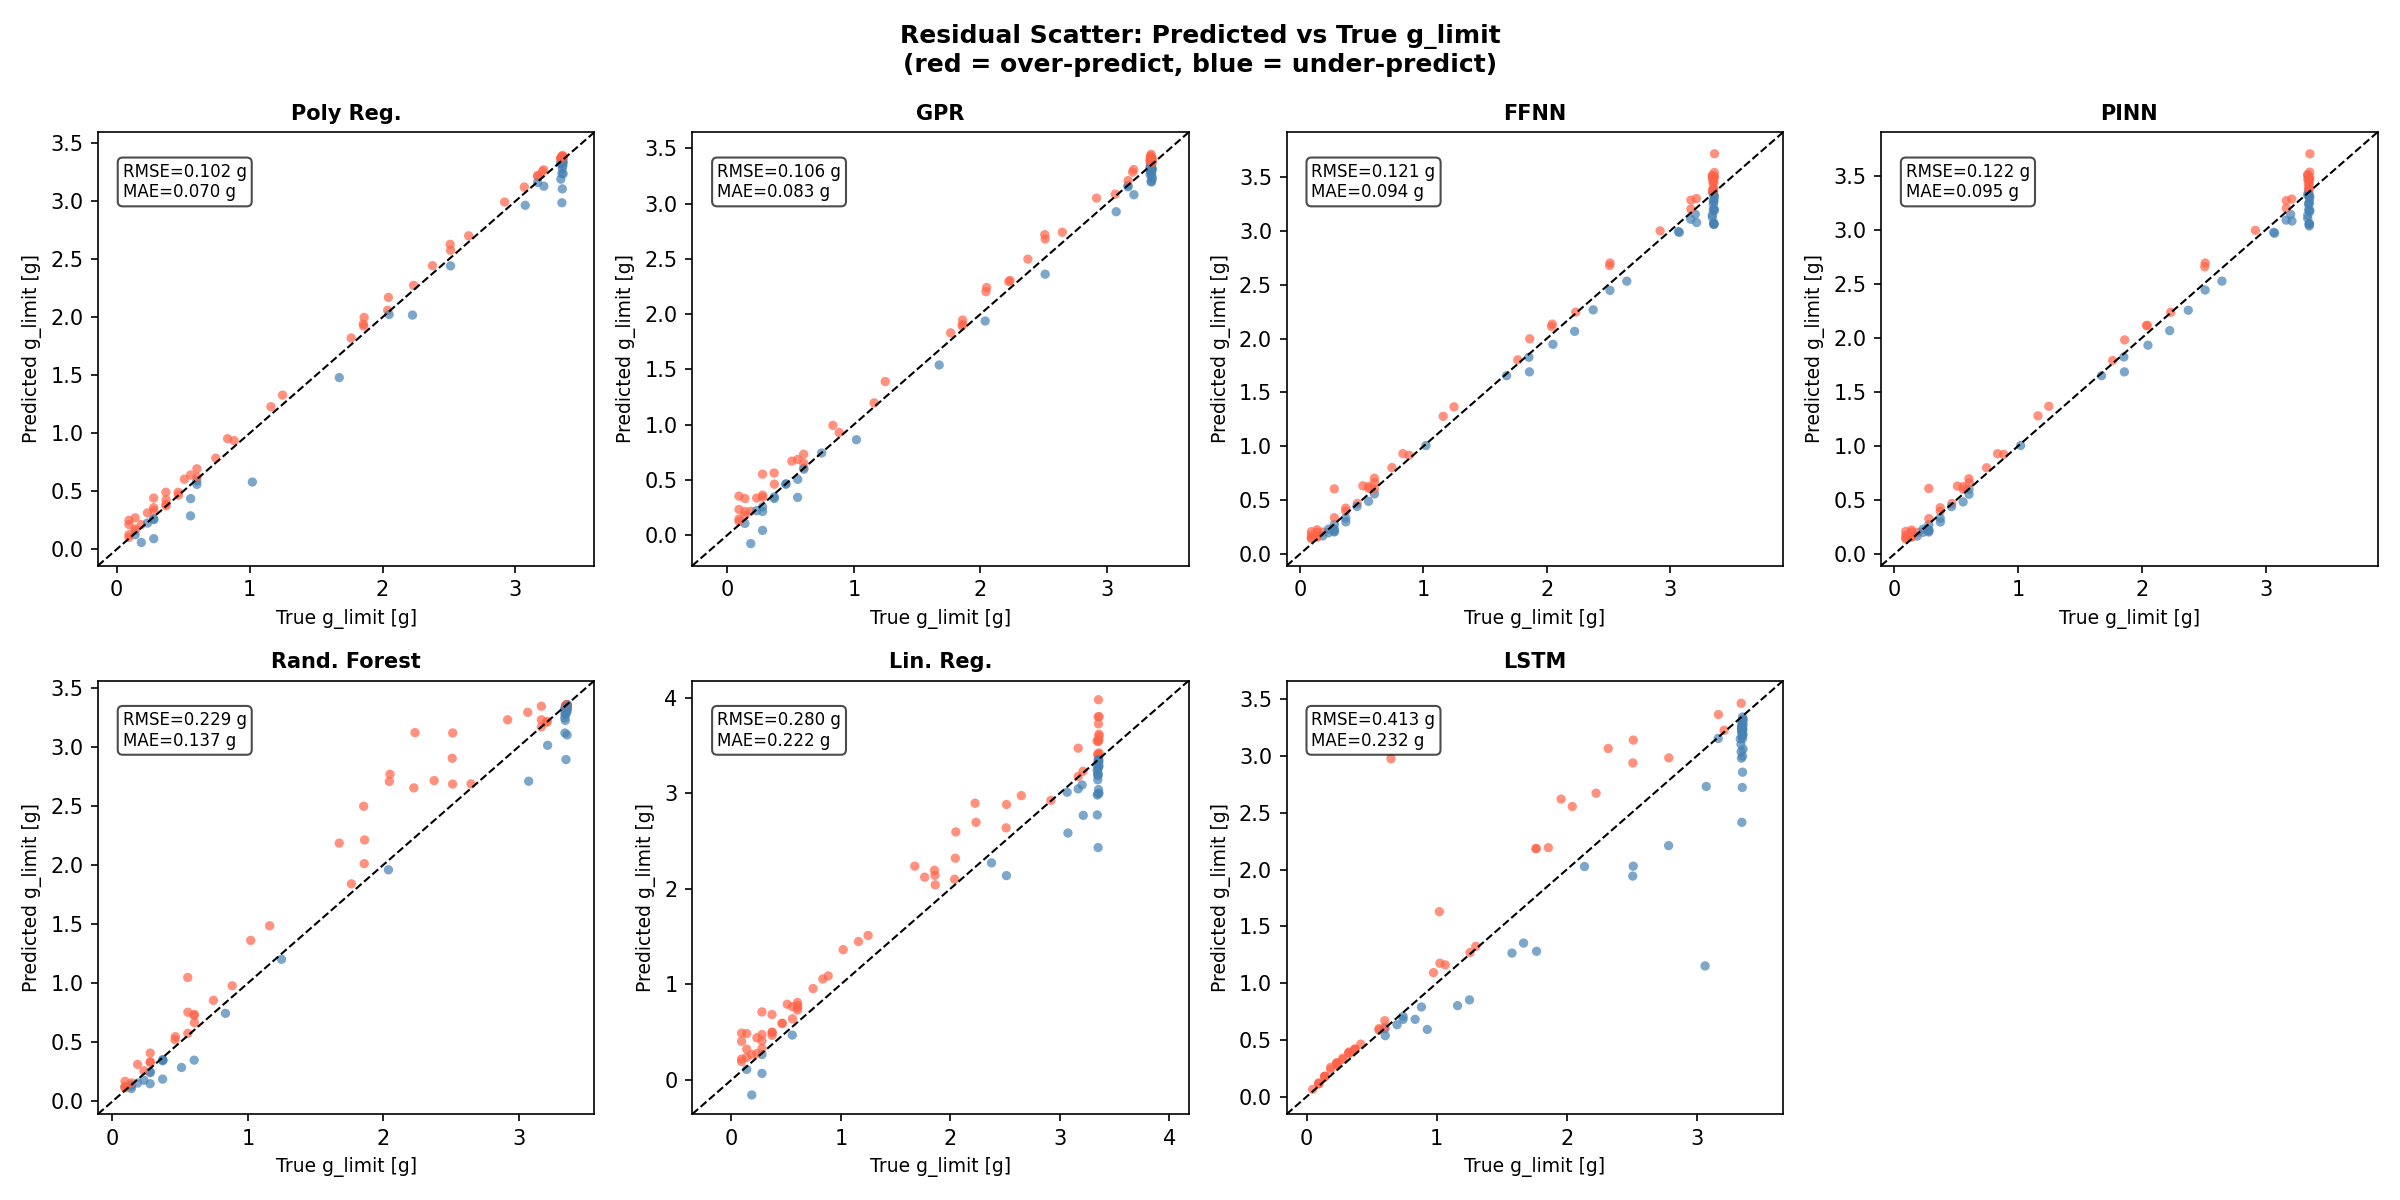
\includegraphics[width=\textwidth]{comparison_residuals.png}
  \caption{Side-by-side residual scatter plots for all seven models.}
  \label{fig:app_residuals}
\end{figure}

\begin{figure}[H]
  \centering
  
\includegraphics[width=0.75\textwidth]{pod_variance.png}
  \caption{Proper Orthogonal Decomposition (POD) cumulative variance explained for the
    strain field, used during exploratory feature analysis.}
  \label{fig:app_pod_variance}
\end{figure}

\begin{figure}[H]
  \centering
  
\includegraphics[width=0.75\textwidth]{pod_r2_vs_k.png}
  \caption{Predictive $\Rsq$ using POD-compressed features as a function of the number
    of retained POD modes.}
  \label{fig:app_pod_r2}
\end{figure}

\begin{figure}[H]
  \centering
  
\includegraphics[width=\textwidth]{correlation_matrix.png}
  \caption{Full correlation matrix across all engineered features, Box-Cox transforms, raw
    gauge readings, and the $g$-limit target. High correlations among the log/Box-Cox
    families are expected by construction; the matrix confirms that Box-Cox features
    decorrelate the feature space relative to the raw engineered columns.}
  \label{fig:app_correlation}
\end{figure}

\end{document}
